% Festlegung des Allgemeinen Dokumentenformats
\documentclass[a4paper,12pt,headsepline]{scrartcl}

% Umlaute unter UTF8 nutzen
\usepackage[utf8]{inputenc}

% Variablen
%Variablen welche innerhalb der gesamten Arbeit zur Verfügung stehen sollen
\newcommand{\titleDocument}{Regenvorhersage mit Neuronalen Netzen und die Visualisierung dieser in einer App}
\newcommand{\subjectDocument}{MSI AS - Master Informatik, Autonome Systeme}


% weitere Pakete
% Grafiken aus PNG Dateien einbinden
\usepackage{graphicx}
\usepackage{float}
\usepackage{subfig}
\usepackage{multirow}
%\usepackage{wrapfig}
% aus SVG
\usepackage{svg}

% Deutsche Sonderzeichen und Silbentrennung nutzen
\usepackage[ngerman]{babel}

% Eurozeichen einbinden
\usepackage[right]{eurosym}

% Zeichenencoding
\usepackage[T1]{fontenc}

\usepackage{lmodern}

% floatende Bilder ermöglichen
%\usepackage{floatflt}

% mehrseitige Tabellen ermöglichen
\usepackage{longtable}

% Unterstützung für Schriftarten
%\newcommand{\changefont}[3]{ 
%\fontfamily{#1} \fontseries{#2} \fontshape{#3} \selectfont}

% Packet für Seitenrandabständex und Einstellung für Seitenränder
\usepackage{geometry}
\geometry{left=3cm, right=3cm, top=2.5cm, bottom=2cm}

% Paket für Boxen im Text
\usepackage{fancybox}

% bricht lange URLs "schön" um
\usepackage[hyphens,obeyspaces,spaces]{url}

% Paket für Textfarben
\usepackage{color}

% Mathematische Symbole importieren
\usepackage{amssymb}

% auf jeder Seite eine Überschrift (alt, zentriert)
%\pagestyle{headings}

% erzeugt Inhaltsverzeichnis mit Querverweisen zu den Abschnitten (PDF Version)
\usepackage[bookmarksnumbered,pdftitle={\titleDocument},hyperfootnotes=false]{hyperref}
%\hypersetup{colorlinks, citecolor=red, linkcolor=blue, urlcolor=black}
%\hypersetup{colorlinks, citecolor=black, linkcolor= black, urlcolor=black}

% neue Kopfzeilen mit fancypaket
\usepackage{fancyhdr} %Paket laden
\pagestyle{fancy} %eigener Seitenstil
\fancyhf{} %alle Kopf- und Fußzeilenfelder bereinigen
\fancyhead[L]{\nouppercase{\leftmark}} %Kopfzeile links
\fancyhead[C]{} %zentrierte Kopfzeile
\fancyhead[R]{\thepage} %Kopfzeile rechts
\renewcommand{\headrulewidth}{0.2pt} %obere Trennlinie
%\fancyfoot[C]{\thepage} %Seitennummer
%\renewcommand{\footrulewidth}{0.4pt} %untere Trennlinie

% für Tabellen
\usepackage{array}

% Runde Klammern für Zitate
%\usepackage[numbers,round]{natbib}

% Festlegung Art der Zitierung - Havardmethode: Abkuerzung Autor + Jahr

%\bibliographystyle{alphadin}
%\bibliography{Hauptdatei}


% Schaltet den zusätzlichen Zwischenraum ab, den LaTeX normalerweise nach einem Satzzeichen einfügt.
%\frenchspacing

% Paket für Zeilenabstand
\usepackage{setspace}

% für Bildbezeichner
\usepackage{capt-of}

% für Stichwortverzeichnis
\usepackage{makeidx}

% für Listings
\usepackage{listings}
\lstset{numbers=left, numberstyle=\tiny, numbersep=5pt, keywordstyle=\color{black}\bfseries, stringstyle=\ttfamily,showstringspaces=false,basicstyle=\footnotesize,captionpos=b}
\lstset{language=java}

% Indexerstellung
\makeindex

% Abkürzungsverzeichnis
\usepackage[german]{nomencl}
\let\abbrev\nomenclature

% Abkürzungsverzeichnis LiveTex Version
% Titel des Abkürzungsverzeichnisses
\renewcommand{\nomname}{Abkürzungsverzeichnis}
% Abstand zwischen Abkürzung und Erläuterung
\setlength{\nomlabelwidth}{.25\textwidth}
% Zwischenraum zwischen Abkürzung und Erläuterung mit Punkten
\renewcommand{\nomlabel}[1]{#1 \dotfill}
% Variation des Abstandes der einzelnen Abkürzungen zu einander
\setlength{\nomitemsep}{-\parsep}
% Index mit Abkürzungen erzeugen
\makenomenclature
%\makeglossary

% Abkürzungsverzeichnis TeTEX Version
% \usepackage[german]{nomencl}
% \makenomenclature
% %\makeglossary
% \renewcommand{\nomname}{Abkürzungsverzeichnis}
% \AtBeginDocument{\setlength{\nomlabelwidth}{.25\columnwidth}}
% \renewcommand{\nomlabel}[1]{#1 \dotfill}
% \setlength{\nomitemsep}{-\parsep}

% Optional: Einzelne Zeilen am Anfang einer Seite unterdrücken (Schusterjungen)
% \clubpenalty = 10000
% Optional: Einzelne Zeilen am Ende einer Seite unterdrücken (Hurenkinder)
% \widowpenalty = 10000
% \displaywidowpenalty = 10000



\usepackage{tikz}

\usetikzlibrary{arrows,decorations.pathmorphing,backgrounds,positioning,fit,petri, decorations.pathreplacing,shadows,calc}

\definecolor{echoreg}{HTML}{2cb1e1}
\definecolor{sublimedg}{HTML}{171813}
\definecolor{lgry}{HTML}{aaaaaa}
\definecolor{mymauve}{rgb}{0.58,0,0.82}

  

\tikzset{%
  cascaded/.style = {%
    general shadow = {%
      shadow scale = 1,
      shadow xshift = -1ex,
      shadow yshift = 1ex,
      draw=black,
      thick,
      fill = white},
    general shadow = {%
      shadow scale = 1,
      shadow xshift = -1ex,
      shadow yshift = 1ex,
      draw=black,
      thick,
      fill = white},
    general shadow = {%
      shadow scale = 1,
      shadow xshift = -.5ex,
      shadow yshift = .5ex,
      draw=black,
      thick,
      fill = white},
    fill = white, 
    draw,
    thick}}
    
\tikzset{%
  cascadedd/.style = {%
    general shadow = {%
      shadow scale = 1,
      shadow xshift = -4.5ex,
      shadow yshift = 4.5ex,
      draw=black,
      thick,
      fill = white},
    general shadow = {%
      shadow scale = 1,
      shadow xshift = -4ex,
      shadow yshift = 4ex,
      draw=black,
      thick,
      fill = white},
    general shadow = {%
      shadow scale = 1,
      shadow xshift = -3.5ex,
      shadow yshift = 3.5ex,
      draw=black,
      thick,
      fill = white},
    general shadow = {%
      shadow scale = 1,
      shadow xshift = -3ex,
      shadow yshift = 3ex,
      draw=black,
      thick,
      fill = white},
    general shadow = {%
      shadow scale = 1,
      shadow xshift = -2.5ex,
      shadow yshift = 2.5ex,
      draw=black,
      thick,
      fill = white},
    general shadow = {%
      shadow scale = 1,
      shadow xshift = -2ex,
      shadow yshift = 2ex,
      draw=black,
      thick,
      fill = white},
    general shadow = {%
      shadow scale = 1,
      shadow xshift = -1.5ex,
      shadow yshift = 1.5ex,
      draw=black,
      thick,
      fill = white},
    general shadow = {%
      shadow scale = 1,
      shadow xshift = -1ex,
      shadow yshift = 1ex,
      draw=black,
      thick,
      fill = white},
    general shadow = {%
      shadow scale = 1,
      shadow xshift = -.5ex,
      shadow yshift = .5ex,
      draw=black,
      thick,
      fill = white},
    fill = white, 
    draw,
    thick}}
    
\tikzset{%
  cascadeddd/.style = {%
    general shadow = {%
      shadow scale = 1,
      shadow xshift = -9ex,
      shadow yshift = 9ex,
      draw=black,
      thick,
      fill = white},
    general shadow = {%
      shadow scale = 1,
      shadow xshift = -8.5ex,
      shadow yshift = 8.5ex,
      draw=black,
      thick,
      fill = white},
    general shadow = {%
      shadow scale = 1,
      shadow xshift = -8ex,
      shadow yshift = 8ex,
      draw=black,
      thick,
      fill = white},
    general shadow = {%
      shadow scale = 1,
      shadow xshift = -7.5ex,
      shadow yshift = 7.5ex,
      draw=black,
      thick,
      fill = white},
    general shadow = {%
      shadow scale = 1,
      shadow xshift = -7ex,
      shadow yshift = 7ex,
      draw=black,
      thick,
      fill = white},
    general shadow = {%
      shadow scale = 1,
      shadow xshift = -6.5ex,
      shadow yshift = 6.5ex,
      draw=black,
      thick,
      fill = white},
    general shadow = {%
      shadow scale = 1,
      shadow xshift = -6ex,
      shadow yshift = 6ex,
      draw=black,
      thick,
      fill = white},
    general shadow = {%
      shadow scale = 1,
      shadow xshift = -5.5ex,
      shadow yshift = 5.5ex,
      draw=black,
      thick,
      fill = white},
    general shadow = {%
      shadow scale = 1,
      shadow xshift = -5ex,
      shadow yshift = 5ex,
      draw=black,
      thick,
      fill = white},
    general shadow = {%
      shadow scale = 1,
      shadow xshift = -4.5ex,
      shadow yshift = 4.5ex,
      draw=black,
      thick,
      fill = white},
    general shadow = {%
      shadow scale = 1,
      shadow xshift = -4ex,
      shadow yshift = 4ex,
      draw=black,
      thick,
      fill = white},
    general shadow = {%
      shadow scale = 1,
      shadow xshift = -3.5ex,
      shadow yshift = 3.5ex,
      draw=black,
      thick,
      fill = white},
    general shadow = {%
      shadow scale = 1,
      shadow xshift = -3ex,
      shadow yshift = 3ex,
      draw=black,
      thick,
      fill = white},
    general shadow = {%
      shadow scale = 1,
      shadow xshift = -2.5ex,
      shadow yshift = 2.5ex,
      draw=black,
      thick,
      fill = white},
    general shadow = {%
      shadow scale = 1,
      shadow xshift = -2ex,
      shadow yshift = 2ex,
      draw=black,
      thick,
      fill = white},
    general shadow = {%
      shadow scale = 1,
      shadow xshift = -1.5ex,
      shadow yshift = 1.5ex,
      draw=black,
      thick,
      fill = white},
    general shadow = {%
      shadow scale = 1,
      shadow xshift = -1ex,
      shadow yshift = 1ex,
      draw=black,
      thick,
      fill = white},
    general shadow = {%
      shadow scale = 1,
      shadow xshift = -.5ex,
      shadow yshift = .5ex,
      draw=black,
      thick,
      fill = white},
    fill = white, 
    draw,
    thick}}


\tikzset{%
  cascaded3/.style = {%
    general shadow = {%
      shadow scale = 1,
      shadow xshift = -9ex,
      shadow yshift = 9ex,
      draw=black,
      thick,
      fill = white},
    general shadow = {%
      shadow scale = 1,
      shadow xshift = -8.5ex,
      shadow yshift = 8.5ex,
      draw=black,
      thick,
      fill = white},
    general shadow = {%
      shadow scale = 1,
      shadow xshift = -8ex,
      shadow yshift = 8ex,
      draw=black,
      thick,
      fill = white},
    general shadow = {%
      shadow scale = 1,
      shadow xshift = -7.5ex,
      shadow yshift = 7.5ex,
      draw=black,
      thick,
      fill = white},
    general shadow = {%
      shadow scale = 1,
      shadow xshift = -7ex,
      shadow yshift = 7ex,
      draw=black,
      thick,
      fill = white},
    general shadow = {%
      shadow scale = 1,
      shadow xshift = -6.5ex,
      shadow yshift = 6.5ex,
      draw=black,
      thick,
      fill = white},
    general shadow = {%
      shadow scale = 1,
      shadow xshift = -6ex,
      shadow yshift = 6ex,
      draw=black,
      thick,
      fill = white},
    general shadow = {%
      shadow scale = 1,
      shadow xshift = -5.5ex,
      shadow yshift = 5.5ex,
      draw=black,
      thick,
      fill = white},

    fill = white, 
    draw,
    thick}}


\tikzset{
test/.style = {%
    general shadow = {%
      shadow scale = 1,
      shadow xshift = -9ex,
      shadow yshift = 9ex,
      draw=black,
      thick,
      fill = white}
      }}


\tikzset{
slimconv/.style = {rectangle, 
  dashed,
  draw=sublimedg, 
  fill=cyan,  
  fill opacity=0.5,
  very thin, 
  minimum width=0.1em, 
  minimum height=12em
      }}


\let\oldquote\quote
\let\endoldquote\endquote
\renewenvironment{quote}[2][]
  {\if\relax\detokenize{#1}\relax
     \def\quoteauthor{#2}%
   \else
     \def\quoteauthor{#2~---~#1}%
   \fi
   \oldquote}
  {\par\nobreak\smallskip\hfill(\quoteauthor)%
   \endoldquote\addvspace{\bigskipamount}}
   %\usepackage{wrapfig}

\newpage

\begin{document}
% hier werden die Trennvorschläge inkludiert
%hier müssen alle Wörter rein, welche Latex von sich auch nicht korrekt trennt bzw. bei denen man die genaue Trennung vorgeben möchte
\hyphenation{
Film-pro-du-zen-ten
Lux-em-burg
Soft-ware-bau-steins
zeit-in-ten-siv
}


% Schriftart Helvetica verwenden
%\usepackage{helvet}
%\renewcommand\familydefault{\sfdefault}

% Titelseite %
\thispagestyle{empty}


\begin{figure}[t]
 \centering
 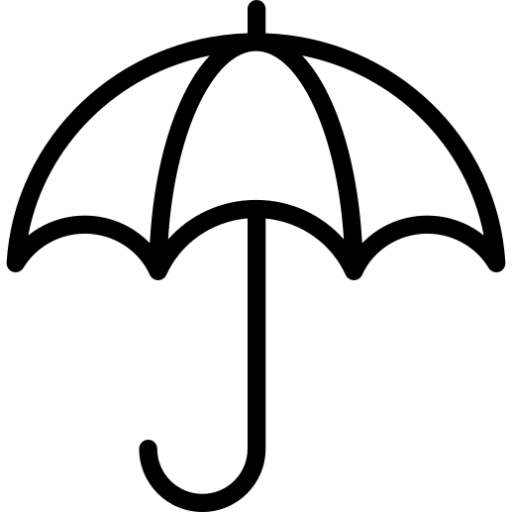
\includegraphics[width=0.2\textwidth]{abb/regenschirm}
\end{figure}


\begin{verbatim}


\end{verbatim}

\begin{center}
\Large{HTWG Konstanz}\\
\end{center}

\begin{center}
\Large{Fakultät für Informatik}
\end{center}
\begin{verbatim}




\end{verbatim}
\begin{center}
\textbf{\LARGE{DeepRain}} \\
\vspace{1cm}
\doublespacing
\textbf{\LARGE{\titleDocument}}\\
\singlespacing
\begin{verbatim}

\end{verbatim}
\textbf{{~\subjectDocument}}
\end{center}
\begin{verbatim}

\end{verbatim}
\begin{center}

\end{center}
\begin{verbatim}


\end{verbatim}
\begin{flushleft}
\begin{tabular}{llll}
\textbf{Autoren:} & & Simon Christofzik& \\
& & Paul Sutter& \\
& & Till Reitlinger \\
& & \\
\textbf{Version vom:} & & \today &\\
& & \\
\textbf{Betreuer:} & & Prof. Dr. Oliver Dürr &\\
\end{tabular}
\end{flushleft}


% römische Numerierung
\pagenumbering{roman}

% 1.5 facher Zeilenabstand
\onehalfspacing

\newpage


% Einleitung / Abstract
\thispagestyle{empty}
\section*{Zusammenfassung}
Ziel der Vorliegenden Arbeit ist zu prüfen, ob es mit begrenzten Ressourcen möglich ist eine Regenvorhersage zu berechnen und diese den Nutzern bereitzustellen.
Für die Berechnung der Regenvorhersage wurden Neuronale Netze eingesetzt.
Die hierfür benötigten historischen und aktuellen Radardaten wurden vom Deutschen Wetterdienst bezogen und anschließend analysiert und aufbereitet. 
Des Weiteren wurde eine App entwickelt, in der die Regenvorhersagen visualisiert werden. 
Außerdem bietet Sie die Möglichkeit, bei bevorstehenden Regen, den Benutzer zu benachrichtigen. 

% einfacher Zeilenabstand
\singlespacing

\newpage
% Seitenzählung bei Inhaltsverzeichnis beginnen
\setcounter{page}{1}

% Inhaltsverzeichnis anzeigen
\thispagestyle{empty}
\tableofcontents

\newpage
% das Abbildungsverzeichnis
% Abbildungsverzeichnis soll im Inhaltsverzeichnis auftauchen
\addcontentsline{toc}{section}{Abbildungsverzeichnis}
% Verion 1: Abbildungsverzeichnis MIT führender Nummberierung endgueltig anzeigen
\listoffigures

% Verion 2: Abbildungsverzeichnis OHNE führende Nummberierung endgueltig anzeigen
%\begingroup
%\renewcommand\numberline[1]{}
%\listofs
%\endgroup


% das Tabellenverzeichnis
%\newpage
% Tabellenverzeichnis soll im Inhaltsverzeichnis auftauchen
%\addcontentsline{toc}{section}{Tabellenverzeichnis}
% \fancyhead[L]{Abbildungsverzeichnis / Abkürzungsverzeichnis} %Kopfzeile links
% Tabellenverzeichnis endgültig anzeigen
%\listoftables

%% WORKAROUND für Listings
%\makeatletter% --> De-TeX-FAQ
%\renewcommand*{\lstlistoflistings}{%
%  \begingroup
%    \if@twocolumn
%      \@restonecoltrue\onecolumn
%    \else
%      \@restonecolfalse
%    \fi
%    \lol@heading
%    \setlength{\parskip}{\z@}%
%    \setlength{\parindent}{\z@}%
%    \setlength{\parfillskip}{\z@ \@plus 1fil}%
%    \@starttoc{lol}%
%    \if@restonecol\twocolumn\fi
%  \endgroup
%}
%\makeatother% --> \makeatletter
% das Listingverzeichnis
%\newpage
% Listingverzeichnis soll im Inhaltsverzeichnis auftauchen
%\addcontentsline{toc}{section}{Listingverzeichnis}
%\fancyhead[L]{Listingverzeichnis} %Kopfzeile links
%\renewcommand{\lstlistlistingname}{Listingverzeichnis}
%\lstlistoflistings
%%%%

% das Abkürzungsverzeichnis
\newpage
% Abkürzungsverzeichnis soll im Inhaltsverzeichnis auftauchen
\addcontentsline{toc}{section}{Abkürzungsverzeichnis}
% das Abkürzungsverzeichnis ausgeben
\fancyhead[L]{Abkürzungsverzeichnis} %Kopfzeile links
\nomenclature{UGC}{User Generated Content}
\nomenclature{CSS}{Cascading Style Sheets}
\nomenclature{JS}{JavaScript}
\nomenclature{SQL}{Structured Query Language}
\nomenclature{GPL}{GNU General Public License}
\nomenclature{GNU}{GNU is not Unix}
\nomenclature{LGPL}{GNU Lesser General Public License}
\nomenclature{XMPP}{Extensible Messaging and Presence Protocol}
\nomenclature{IM}{Instant Message}
\nomenclature{CMS}{Content Management System}
\nomenclature{RSS}{Really Simple Syndication}
\nomenclature{JSON}{JavaScript Object Notation}
\nomenclature{HTML}{Hypertext Markup Language}
\nomenclature{TDD}{Test-driven development}
\nomenclature{GUI}{Graphical User Interface}
\nomenclature{KPI}{Key Performance Indicator}
\nomenclature{WWW}{World Wide Web}
\nomenclature{OCR}{Optical Character Recognition}
\nomenclature{ERM}{Entity Relationship Modell}



\nomenclature{KNN} {Künstliches neuronales Netz}
\printnomenclature[3cm]


%%%%%%% EINLEITUNG %%%%%%%%%%%%
\newpage
\fancyhead[L]{\nouppercase{\leftmark}} %Kopfzeile links

% 1,5 facher Zeilenabstand
\onehalfspacing

% arabische Seitennummerierung ab hier
\pagenumbering{arabic}



\nocite{*} % adds all references without citations to bibliography
\bibliographystyle{apalike}
\bibliography{Hauptdatei}


\section{Gesamtsystem}\label{gesamtsystem}
In folgender Abbildung ist die komplette Datenpipeline von dem Server des DWD bis zur Darstellung in der App zu sehen.  

\begin{figure}[htb]
 \centering
 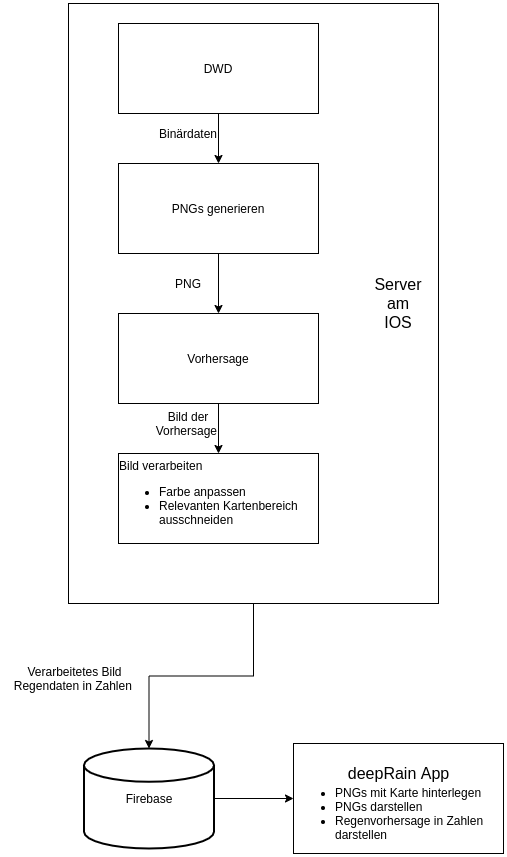
\includegraphics[width=0.6\textwidth,angle=0]{abb/Gesamtsystem}
 \caption[Das Gesamtsystem]{Das Gesamtsystem}
\label{fig:Beschreibung}
\end{figure}

Der DWD stellt alle fünf Minuten die neusten Regendaten für Deutschland im Binär Format auf dem Opendata Server des DWD zur Verfügung. 
Diese werden heruntergeladen und in der Datenaufbereitung verwendet um PNGs zu generieren (Siehe Kapitel “Datenaufbereitung”). 
Dieses PNGs werden im Anschluss verwendet um eine Regenvorhersage zu machen (Siehe Kapitel “Regenvorhersage / Netze”). 
Der Output der Regenvorhersage ist wieder ein PNG. 
Dieses PNG wird in der Firebase gespeichert und auf allen Geräten mit der installierten App angezeigt (Siehe Kapitel “App und Datenbank”). 
Der Übersichtlichkeit halber haben wir das gesamte Projekt in die drei Komponenten “Datenbeschaffung |\& Vorverarbeitung”, “Vorhersage” und 
“App |\& Datenbankhandling” aufgeteilt.  
Die Komponente “Datenbeschaffung |\& Vorverarbeitung” reicht vom Download der Binär - Daten beim DWD bis zu den daraus generierten PNG’s. 
In der Komponente “Vorhersage” werden die Regenvorhersage mithilfe von neuronalen Netzen gemacht. In der Komponente “App |\& Datenbankhandling” 
geht es um das Datenmanagement mit der Firebase, und um die App welche die Daten darstellt.  
(Hier sollten wir gegen Ende des Projektes eventuell noch ein bisschen genauer beschreiben wie das alles genau funktioniert. 
Das wird unseren Nachfolgern sehr stark helfen um sich schnell einzuarbeiten)  

\section{Die Daten}\label{die daten}
Die Datengrundlage für die Netze werden von dem DWD in Form des Radar Online Aneichungs verfahren (RADOLAN) zur Verfügung gestellt. Das RADOLAN verfahren kombiniert die Messungen der 18 Radarstation und den punktuellen Messungen von über 2000 Bodenniederschlagsstationen (https://www.dwd.de/DE/leistungen/radolan/radolan.html). Eine dieser Bodenniederschlagsstationen befindet sich in Konstanz. 

\begin{figure}[htb]
 \centering
 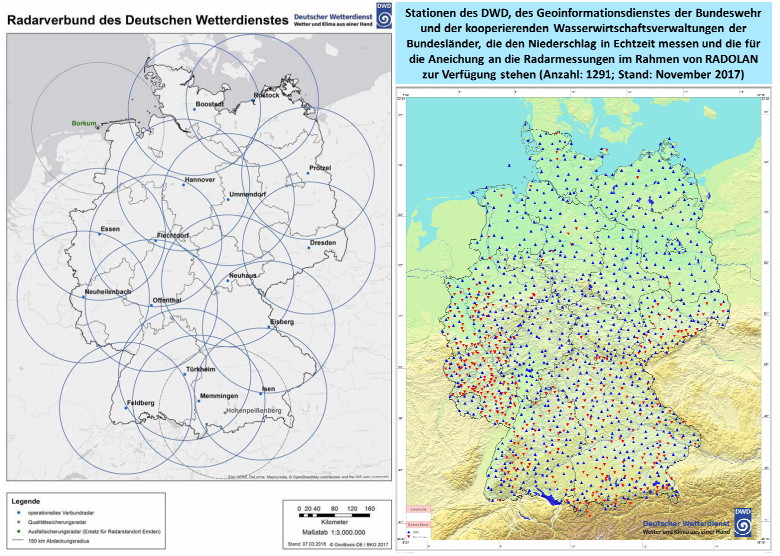
\includegraphics[width=0.6\textwidth,angle=0]{abb/daten_stationsuebersicht}
 \caption[Stationen Übersicht]{Übersicht über alle Boden und Radarstationen}
\label{fig:daten_stationsuebersicht}
\end{figure}

Um die Qualität der aus den RADAR Daten gewonnenen PNGs zu überprüfen, wurden die PNGs mit den Niederschlagsdaten von der Bodenstation in Konstanz verglichen. Die Daten der Station stehen in ein und zehn minütiger Auflösung zur Verfügung. Da sich herausstellte, dass bei der ein minütigen Auflösung Daten Fehlen, wurden die Daten der 10 minütigen Auflösung verwendet um die PNGs zu validieren. 
Die RADOLAN Daten für die Netze werden über den Opendata Server vom DWD zur Verfügung gestellt. Die Binärdaten werden je nach Jahr in Form eines 1100x900 oder 900x900 Pixel Gitter über Deutschland gelegt.  Dabei entspricht jeder Pixel 1km x 1km. Jeder Pixel in dem Pixel Koordinatensystem hat dabei zugehörige Höhen und Breitengrad Koordinaten. In folgender Abbildung ist der Aufbau der Binärdaten zu sehen.

\begin{figure}[h]
 \centering
 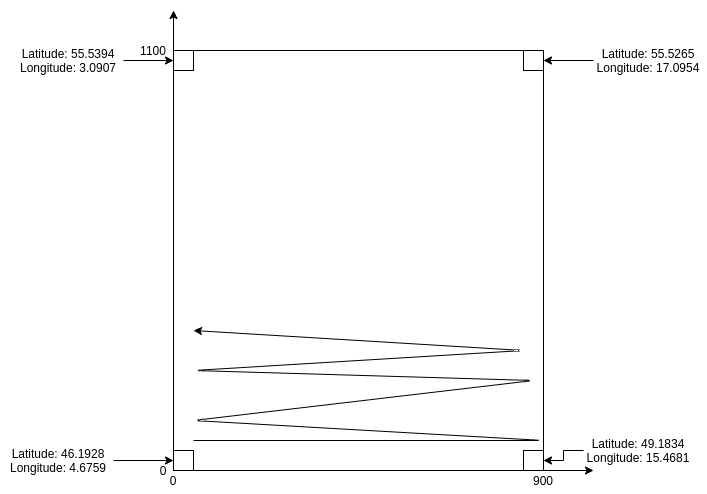
\includegraphics[width=0.8\textwidth,angle=0]{abb/radolan_koordinatensystem_aufbau}
 \caption[Aufbau des Koordinatensystems von Binärdaten]{Der Aufbau des Koordinatensystems der Radar Daten}
\label{fig:radolan_koordinatensystem_aufbau}
\end{figure}

Wie zu sehen ist, befinden sich der Pixel (0|0) in der Ecke unten links. Bei der Datenvorverarbeitung wird das Array mit den Pixeln jedoch von oben Links beginnend gefüllt, was bei dem entstehenden PNG  zu einer Spiegelung von 90 grad um die vertikale Achse führt (Siehe Kapitel Datenaufbereitung). 
Des weiteren ist zu beachten, dass die Breitengrade in den Ecken nicht übereinstimmen. So hat die Ecke unten Links einen größeren Breitengrad als die Ecke oben Links. Das gleiche ist auch bei den Höhengraden zu beobachten. Die Ursache hierfür ist die Transformation der Daten von einer 3D Kugel auf eine 2D Karte. In Abbildung \ref{fig:karte_abdeckung_daten} ist das daraus resultierende Ergebnis abgebildet. 

\begin{figure}[H]
 \centering
 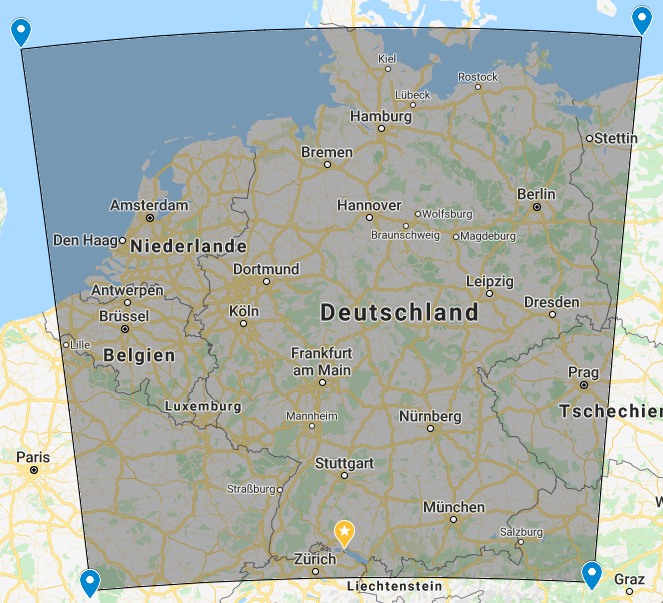
\includegraphics[width=0.6\textwidth,angle=0]{abb/karte_abdeckung_daten}
 \caption[Von Daten abgedeckte Fläche]{Die von den Daten abgedeckte Fläche auf einer 2D Karte}
\label{fig:karte_abdeckung_daten}
\end{figure}

\section{Die Datenaufbereitung}\label{die datenaufbereitung}
Die vom Deutschen Wetterdienst (im Folgenden DWD abgekürzt) in fünf minütiger Auflösung bereitgestellten Radardaten, müssen für das Training der Netze und deren Vorhersage in ein Bildformat umgewandelt werden.
Bei den bereits umgewandelten Bildern viel während der Entwicklung der Baseline auf, dass die Bilder weit weniger Regentage abbilden als es tatsächlich regnet. Daraufhin wurde das bisher vorgenommene Preprocessing evaluiert. Um die Radardaten in ein Bild umzuwandeln, muss jeder Radardatenpunkt in ein Pixelfarbwert transformiert werden. Bisher wurde dafür ein Sakalierungsfaktor berechnet mit dem jeder Radardatenpunkt multipliziert wurde. Der Faktor ergab sich aus dem zur Verfügung stehenden Wertebereich (0 bis 255), welcher durch den Maximalwert der Radardaten geteilt wurde. So erhält man transformierte Radarwerte in einem Bereich von 0 bis 255.
Anschließend folgte eine Inspizierung der Daten. Hierfür wurde exemplarisch die Radardaten von Juni 2016 herangezogen.

\begin{figure}[h]
 \centering
 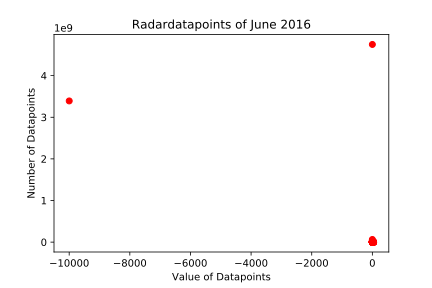
\includegraphics[width=0.6\textwidth,angle=0]{abb/Radardatapoints_of_June_2016}
 \caption[Datenaufbereitung]{Häufigkeitsverteilung der Regendaten}
\label{fig:datenaufbereitung}
\end{figure}

Geplottet werden alle auftretenden Werte sowie dessen Häufigkeit. Hierbei stechen zwei Ausreißer hervor, welche sehr viel häufiger vorkommen als die restlichen Werte. Der Wert –9999 steht dabei dafür, dass keine Daten verfügbar sind und der zweite Ausreißer ist bei 0, was für “kein Regen” steht. In dem folgenden Plot werden die beiden Ausreißer gefiltert, da die relevanten Informationen in den restlichen Datenpunkten stecken.

\begin{figure}[h]
 \centering
 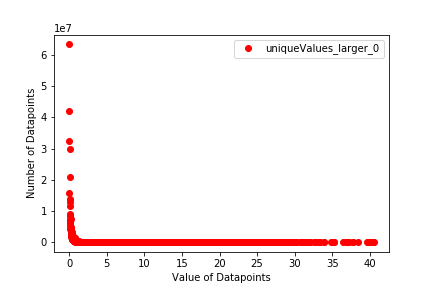
\includegraphics[width=0.6\textwidth,angle=0]{abb/Radardatapoints_of_June_2016_larger0}
 \caption[Datenaufbereitung]{Häufigkeitsverteilung der Regendaten größer null}
\label{fig:datenaufbereitung}
\end{figure}

In diesem Plot dargestellt sind die Radardaten bei denen es regnet. Es wird deutlich, dass ein Großteil der Datenpunkte klein ist. Der Mittelwert liegt bei 0,1744 und zeigt das Problem der bestehenden preprocessing Methode: Radardatenpunkte deren Wert auch nach der Multiplikation mit dem berechneten Skalierungsfaktor kleiner eins sind werden zu null. Aufgrund der vorliegenden Datenverteilung führt das zu einem erheblichen Fehler weshalb eine andere Methode entwickelt werden muss.
Die beiden folgenden Plots zeigen verschiedene Perzentile und machen so die Datenverteilung deutlich.

\begin{figure}[h]
 \centering
 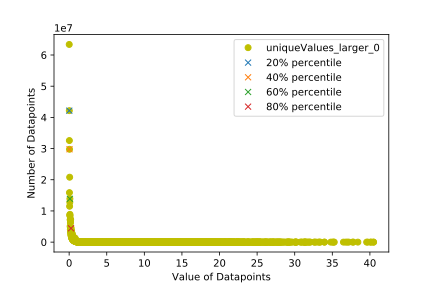
\includegraphics[width=0.6\textwidth,angle=0]{abb/Radardatapoints_of_June_2016_larger0_percentiles}
 \caption[Datenaufbereitung]{Häufigkeitsverteilung der Regendaten mit Perzentilen}
\label{fig:datenaufbereitung}
\end{figure}

\begin{figure}[h]
 \centering
 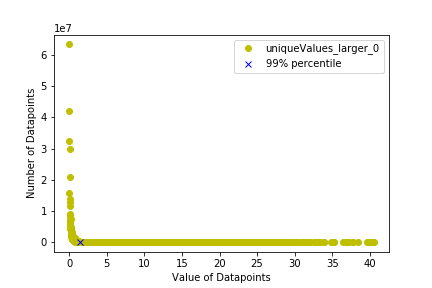
\includegraphics[width=0.6\textwidth,angle=0]{abb/Radardatapoints_of_June_2016_larger0_99percentile}
 \caption[Datenaufbereitung]{Häufigkeitsverteilung der Regendaten mit 99% Perzentil}
\label{fig:datenaufbereitung}
\end{figure}

Das 99 Prozent-Perzentil beinhaltet 138 verschiedene Werte. Wenn jedem dieser Werte ein Farbwert zugeordnet wird, werden 99 Prozent der daten bereits abgebildet und es verbleit ein Wertebereich von 117 mit welchem das letzte Prozent der Daten dargestellt werden kann.
Der folgende Plot zeigt die Verteilung der noch verbleibenden Daten.

\begin{figure}[h]
 \centering
 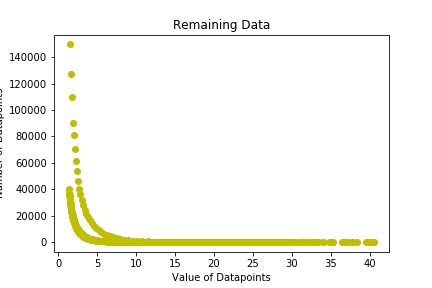
\includegraphics[width=0.6\textwidth,angle=0]{abb/Radardatapoints_of_June_2016_RemainingData}
 \caption[Datenaufbereitung]{Regendaten außerhalb des 99% Perzentils}
\label{fig:datenaufbereitung}
\end{figure}

Noch immer befindet sich der größte Teil der Datenpunkte im kleinem Wertebereich. Da für die verbleibenden Daten eine lineare Transformation ähnlich dem bereits bestehenden preprocessing Vorgang eingesetzt wird, entstehen Rundungsfehler. Da für die Berechnung des Skalierungsfaktors auch nicht der tatsächliche Maximalwert genutzt wird werden Werte die nach der Transformation über 255 sind auf 255 gesetzt. Diese Fehler sind verkraftbar, da es zum einen wichtiger ist alle Datenpunkte abzubilden und zum anderen die Auflösung der verschiedenen Regenstärken immer noch höher ist, als die der menschlichen Wahrnehmung.
Radardaten welche transformiert werden müssen:

\begin{figure}[h]
 \centering
 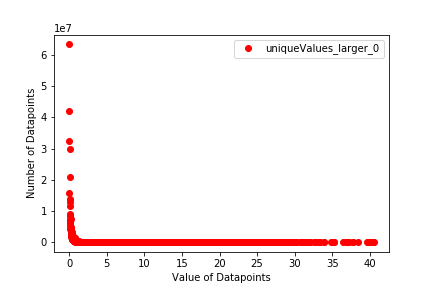
\includegraphics[width=0.6\textwidth,angle=0]{abb/Radardatapoints_of_June_2016_larger0}
 \caption[Datenaufbereitung]{Häufigkeitsverteilung der Regendaten größer null vor der Transformation}
\label{fig:datenaufbereitung}
\end{figure}

Die transformierten Daten befinden sich in einem Wertebereich von 0 bis 255.

\begin{figure}[h]
 \centering
 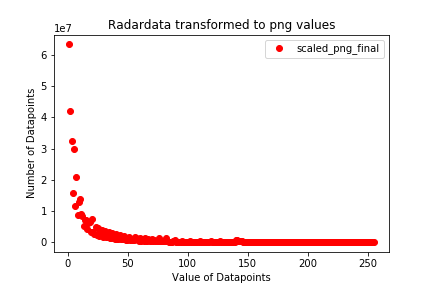
\includegraphics[width=0.6\textwidth,angle=0]{abb/Radardatapoints_of_June_2016_TransformedToPNG}
 \caption[Datenaufbereitung]{Häufigkeitsverteilung der Regendaten größer null nach der Transformation}
\label{fig:datenaufbereitung}
\end{figure}

Rekonstruiert man aus dem PNG Daten wieder die Radardaten ergibt sich der folgende Plot. Die quantitativ wiederhergestellte Anzahl der Datenpunkte beträgt 100%. Von den beschriebenen Fehlern macht sich im Plot vor allem letzterer im Plot bemerkbar. Werte größer als der für diesen Plot angenommenem Maximalwert von 21,39 wurden bei der Transformation auf 255 gesetzt und lassen sich daher nicht mehr konstruieren und erhalten deshalb den Wert 21,39.

\begin{figure}[h]
 \centering
 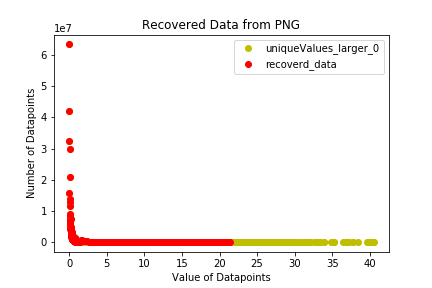
\includegraphics[width=0.6\textwidth,angle=0]{abb/Radardatapoints_of_June_2016_RecoveredData}
 \caption[Datenaufbereitung]{Vergleich zwischen Ausgangsverteilung und Verteilung aus wiederhergestellten Daten}
\label{fig:datenaufbereitung}
\end{figure}


\newpage

\section{Die neuronalen Netze}\label{die neuronalen netze}

Die Regenvorhersage mit Hilfe von künstlichen neuronalen Netzen möchten wir mit einem Zitat einführen.
Der Nobelpreisträge Richard P. Feynman ist in einem Gespräch mit einem nicht namentlich erwähnten Laien wobei es um die Existenz fliegender Untertassen geht. Feynman trifft die Aussage, dass es sehr unwahrscheinlich ist, dass es fliegende Untertassen gibt. Der Laie antwortet darauf, dass das sehr unwissenschaftlich sei, worauf Feynman erwiedert:

\begin{quote}{Richard P. Feynman}
''...But that is the way that is scientific. It is scientific only to say what is more likely and what less likely, and not to be proving all the time the possible and impossible.''  
\end{quote}

\noindent Treffend wird in dem Gespräch von Feynman erläutert, dass der wissenschaftliche Weg eine Wahrscheinlichkeit beinhaltet, die Auskunft über das Eintreten eines Ereignisses gibt. Wir werden für die Regenvorhersage also eine probabilistische Aussage treffen. Dies bedeutet insbesondere, dass eine Verteilung für die Regenvorhersage geschätzt wird, durch die eine Aussage über die Regenwahrscheinlichkeit und auch die Wahrscheinlichkeit der Intensität getroffen werden kann.\\

\noindent Bei der Regenvorhersage via KNN bekommt das KNN als Input ein Set von Bildern, woraus ein Feld von Parametern geschätzt wird, wodurch in Kombination mit der zugehörigen Verteilung eine 30-minütige Vorhersage generiert werden kann. Dieser Vorgang ist in der nachfolgenden Abbildung skizziert.


\begin{figure}[htb]
 \centering
 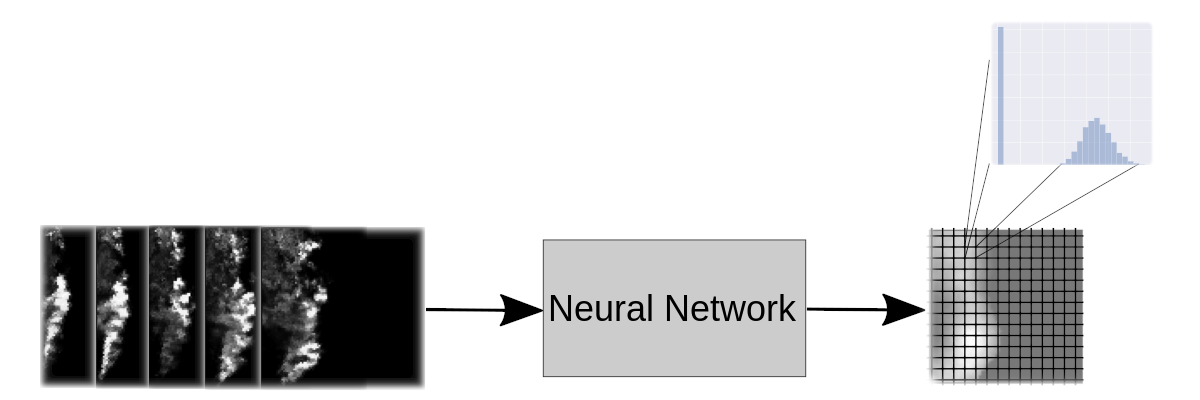
\includegraphics[width=1.0\textwidth,angle=0]{abb/skizzierung_regenvorhersage}
 \caption{Skizzierung der Vorhersage}
\label{fig:Vorhersage_skizze}
\end{figure}

\noindent Wie aus Abbildung \ref{fig:Vorhersage_skizze} hervorgeht, besteht der Ausgang des KNN aus einem Feld von Verteilungen. Diese Verteilungen nehmen wir als unabhängig an.
Die zu schätzende Verteilung ist im vornherein nicht klar, weshalb wir eingangs drei Verteilungen begutachten.
Wir schauen uns die Multinomiale, die Poisson und die negativ Binomial Verteilung an.
Die Poisson und die negativ Binomialverteilung wird allerdings mit der Multinomialen Verteilung gemischt, sodass wir die ''Zero-Inflated negativ Binomial'' bzw. ''Zero-Inflated Poisson'' Verteilung erhalten.
Dies kann so aufgefasst werden, dass wir eine Bernoulli-Verteilung für die binäre Entscheidung über Regen oder kein Regen erhalten. Für den Fall dass Regen vorhergesagt wird, greifen wir auf die Negativ Binomial bzw. Poisson Verteilung zurück.
\\

\subsection{Netzwerk Topologie}

\noindent Wir schauen uns zwei verschiedene Netzwerarchitekturen an. Hierbei passen wir uns den Beschränkungen der uns zur Verfügung stehenden Hardware an.
Uns steht eine Geforce 2060 Super mit 8GB VRAM zur Verfügung. Die Netzwertopologie ist auf die Größe des VRAMS beschränkt, wir werden unser Netzwerk also auf diese Größe beschränken. Die Größe der Eingangsbilder setzen wir auf 96x96 Pixel fest und die Größe der Ausgangsbilder auf 64x64. Die Patches werden um den Pixel, der Konstanz repräsentiert ausgeschnitten.
Alle Netzwerke die wir trainieren haben die Klassifikationsschicht gemeinsam, unterscheiden sich jedoch für die verschiedenen Verteilungen.\\

\begin{figure}[h]
 \centering
\begin{tikzpicture}[inputnode/.style={circle, draw=black!60, fill=green!5,  minimum size=10mm},
input/.style={circle},
outputnode/.style={circle},
]


\node[rectangle, 
dashed, 
draw=sublimedg, 
fill=gray,  
fill opacity=0.2,
very thick, 
minimum width=40em, 
minimum height=20.0em] (duh) at (4, 3) {};

\node[input]            (x0)               at (-3,3)         {};

\node[inputnode]        (inputlayer)       at (3,2)         {};
\node[input]            (x4)               at (3,3)         {$\vdots$};
\node[input]            (x2_3)             at (3.5,3)       {256};
\node[inputnode]        (inputlayer_1)     at (3,4)         {};

\node[outputnode]       (outputlayer)      at (6,2)         {};
\node[inputnode]        (x1)               at (0,5)         {};
\node[input]            (x2)               at (0,3)         {$\vdots$};
\node[input]            (x2_2)             at (0,3.5)       {4096};
\node[inputnode]        (x3)           	   at (0,1)         {};


\node[inputnode]        (x5)               at (6,5)         {};
\node[input]            (x6)               at (6,3)         {$\vdots$};
\node[input]            (x2_1)             at (6,3.5)       {4096 x $n$};
\node[inputnode]        (x7)           	   at (6,1)         {};
%\node[inputnode]        (x9)           	   at (10,3)         {};

\node[cascaded,
		minimum width=4em, 
		minimum height=4em] (x9) at (10,3) {64x64};

\draw[-latex] (x1.east) -- node[above] {} (inputlayer.west);
\draw[-latex] (x3.east) -- node[above] {} (inputlayer.west);
\draw[-latex] (x1.east) -- node[above] {} (inputlayer_1.west);
\draw[-latex] (x3.east) -- node[above] {} (inputlayer_1.west);

\draw[-latex] (inputlayer.east) -- node[above] {} (x5.west);
\draw[-latex] (inputlayer.east) -- node[above] {} (x7.west);

\draw[-latex] (inputlayer_1.east) -- node[above] {} (x5.west);
\draw[-latex] (inputlayer_1.east) -- node[above] {} (x7.west);

\draw[-latex] (x0.east) -- node[above] {Flatten} (x2.west);
\draw[-latex] (x6.east) -- node[above] {64x64x$n$} (x9.west);

\end{tikzpicture}
 \caption{Klassifikationsschicht, $n$ variiert hierbei je nach Verteilung. Für die Zero-Inflated Poisson Verteilung ist $n$ gleich 2, für die Zero-Inflated Negativ Binomial Verteilung ist $n$ gleich 3, und für die Multinomiale Verteilung ist $n$ gleich 7  }
\label{fig:classification_layer}
\end{figure}

\newpage
\noindent Wir verwenden zum einen die Unet-Architektur, wie sie von unseren Vorgängern verwendet wird. Diese Architektur ist in der folgenden Abbildung zu sehen.



\begin{figure}[h]
 \centering
\begin{tikzpicture}[thick,scale=0.5, every node/.style={scale=0.5},inputnode/.style={circle, draw=black!60, fill=green!5,  minimum size=10mm},
input/.style={circle},
outputnode/.style={circle},]
	

	% Schicht 1
	\node[input,rotate=90] (top1_txt) at (0.5,-1) {64x64};
	\node[slimconv] (top1) at (1, 1) {5} ;
	\node[slimconv] (top2) at (2.0, 1) {20} ;
	\node[slimconv] (top3) at (3.0, 1) {20};
	\draw[-stealth, very thick] (top1.east) -- (top2);
	\draw[-stealth, very thick] (top2.east) -- (top3);


	% Schicht 2
	\node[input,rotate=90] (top1_txt) at (2.5,-4.25) {32x32};
	\node[slimconv,
			minimum height=6em] (top1_1) at (3.0, -3.5) {25};
	\node[slimconv,
			minimum width=1.5em, 
			minimum height=6em] (top2_1) at (4.0, -3.5) {25};
	\node[slimconv,
			minimum width=1.5em, 
			minimum height=6em] (top3_1) at (5.125, -3.5) {25};
	\draw[-stealth, very thick] (top1_1.east) -- (top2_1);
	\draw[-stealth, very thick] (top2_1.east) -- (top3_1);
	\draw[-stealth, very thick,red] (top3.south) -- (top1_1.north);


	% Schicht 3
	\node[input,rotate=90] (top1_txt) at (4.5,-6.125) {16x16};
	\node[slimconv,
			minimum width=2em, 
			minimum height=3em] (top1_2) at (5.125, -6.0) {25};
	\node[slimconv,
			minimum width=2.5em, 
			minimum height=3em] (top2_2) at (6.75, -6.0) {25};
	\node[slimconv,
			minimum width=2.5em, 
			minimum height=3em] (top3_2) at (8.5, -6.0) {25};

	\draw[-stealth, very thick] (top1_2.east) -- (top2_2);
	\draw[-stealth, very thick] (top2_2.east) -- (top3_2);
	\draw[-stealth, very thick,red] (top3_1.south) -- (top1_2.north);


	% Schicht 4
	\node[input,rotate=90] (top1_txt) at (7.825,-7.75) {8x8};
	\node[slimconv,
			minimum width=2em, 
			minimum height=2em] (top1_3) at (8.5, -7.75) {25};
	\node[slimconv,
			minimum width=3.5em, 
			minimum height=2em] (top2_3) at (10.25, -7.75) {25};
	\node[slimconv,
			minimum width=3.5em, 
			minimum height=2em] (top3_3) at (12.25, -7.75) {25};

	\draw[-stealth, very thick] (top1_3.east) -- (top2_3);
	\draw[-stealth, very thick] (top2_3.east) -- (top3_3);
	\draw[-stealth, very thick,red] (top3_2.south) -- (top1_3.north);



	% Schicht 5
	\node[input,rotate=90] (top1_txt) at (11.25,-9.25) {4x4};
	\node[slimconv,
			minimum width=3.5em, 
			minimum height=1.5em] (top1_4) at (12.25, -9.25) {25};
	\node[slimconv,
			minimum width=3.5em, 
			minimum height=1.5em] (top3_4) at (16.75, -9.25) {25};

	%\draw[-stealth, very thick] (top1_4.east) -- (top3_4) ;
	\draw[-stealth, very thick] (top1_4.east) -- (top3_4);
	\draw[-stealth, very thick,red] (top3_3.south) -- (top1_4.north);

	% Schicht 4 ( UP )

	\node[slimconv,
			minimum width=2em,
			fill=white,
			minimum height=2em] (top4_30) at (15.6, -7.75) {};
	\node[slimconv,
			minimum width=3.5em, 
			minimum height=2em] (top4_31) at (16.75, -7.75) {50};
	\node[slimconv,
			minimum width=3.5em, 
			minimum height=2em] (top5_3) at (19.25, -7.75) {50};
	\node[slimconv,
			minimum width=3.5em, 
			minimum height=2em] (top6_3) at (21.25, -7.75) {50};


	
	\draw[-stealth, very thick,opacity=0.5] (top3_3.east) -- (top4_30.west);
	\draw[-stealth, very thick] (top4_31.east) -- (top5_3);
	\draw[-stealth, very thick] (top5_3.east) -- (top6_3);
	\draw[-stealth, very thick,green] (top3_4.north) -- (top4_31.south);


		% Schicht 3 (UP)
	\node[slimconv,
			minimum width=2em,
			fill=white,
			minimum height=3em] (top4_20) at (20.125, -6.0) {};
	\node[slimconv,
			minimum width=3.5em, 
			minimum height=3em] (top4_21) at (21.25, -6.0) {75};
	\node[slimconv,
			minimum width=2.5em, 
			minimum height=3em] (top5_2) at (23.25, -6.0) {75};
	\node[slimconv,
			minimum width=2.5em, 
			minimum height=3em] (top6_2) at (25, -6.0) {75};


	\draw[-stealth, very thick,opacity=0.5] (top3_2.east) -- (top4_20.west);
	\draw[-stealth, very thick] (top4_21.east) -- (top5_2);
	\draw[-stealth, very thick] (top5_2.east) -- (top6_2);
	\draw[-stealth, very thick,green] (top6_3.north) -- (top4_21.south);

	% Schicht 2
	\node[slimconv,
		minimum width=1.5em,
		fill=white,
		minimum height=6em] (top4_10) at (24.18, -3.5) {};
	\node[slimconv,
			minimum width=2.5em,
			minimum height=6em] (top4_11) at (25.0, -3.5) {100};
	\node[slimconv,
			minimum width=1.5em, 
			minimum height=6em] (top5_1) at (26.5, -3.5) {100};
	\node[slimconv,
			minimum width=1.5em, 
			minimum height=6em] (top6_1) at (27.75, -3.5) {100};

	\draw[-stealth, very thick,opacity=0.5] (top3_1.east) -- (top4_10.west);
	\draw[-stealth, very thick] (top4_11.east) -- (top5_1);
	\draw[-stealth, very thick] (top5_1.east) -- (top6_1);
	\draw[-stealth, very thick,green] (top6_2.north) -- (top4_11.south);



	
	\node[slimconv,fill=white,] (top4_0) at (27.125, 1) {};
	\node[slimconv] (top4_1) at (27.75, 1) {120};
	\node[slimconv] (top5) at (29, 1) {n};
%	\node[slimconv] (top6) at (29.75, 1) {};

	\draw[-stealth, very thick,opacity=0.5] (top3.east) -- (top4_0.west);
	\draw[-stealth, very thick] (top4_1.east) -- (top5);
%	\draw[-stealth, very thick] (top5.east) -- (top6);
	\draw[-stealth, very thick,green] (top6_1.north) -- (top4_1.south);





	\node[input]        (A1)       at (27.75, -8)         {};
	\node[input]        (A2)       at (27.75, -9.5)         {};
	\draw[-stealth, very thick,green] (A2.north) -- node[right,opacity=1.0,black] {Up-Sampling} (A1.south);


	\node[input]        (A3)       at (27.75, -6)         {};
	\node[input]        (A4)       at (27.75, -7.5)         {};
	\draw[-stealth, very thick,red] (A3.south) -- node[right,opacity=1.0,black] {Pooling} (A4.north);



	\node[input]        (A5)       at (27.75, -7.75)         {};
	\node[input]        (A6)       at (30.0, -7.75)         {Conv 3x3};
	\draw[-stealth, very thick,black] (A5.east) -- (A6.west);



	\node[input]        (A7)       at (25.75, -7.75)         {};
	\node[input]        (A8)       at (27.25, -7.75)         {};
	\draw[-stealth, very thick,gray] (A7.east) --node[above,opacity=1.0,black]{Skipping} (A8.west);


\node[rectangle, 
dashed, 
draw=sublimedg, 
fill=gray,  
fill opacity=0.4,
very thick, 
minimum width=5em, 
minimum height=5em] (kl) at (31, 1) {Kl-Schicht};
	\draw[-stealth, very thick] (top5.east) -- (kl.west);

\end{tikzpicture}
 \caption{Abgespekte Version des Unets  }
\label{fig:Unet1}
\end{figure}

\noindent Die abgespekte Version des Unets hat im Gegensatz zur originalen Architektur wesentlich weniger Gewichte.
Hier sind es ca 10 000 trainierbare Gewichte. Hierbei liegt der Hauptteil der Gewichte in der Klassifikationsschicht (Kl-Schicht in Bild \ref{fig:Unet1}).\\


\noindent Eine weitere Architektur die wir begutachten ist ein Mix aus Inception-Layer und CNN-LSTM-Layer. Die Regenvorhersage in unserem Setup wird für gewöhnlich auch als Next-Frame prediction bezeichnet. Aus einem Set aufeinander folgender eingehender Bilder wird eine plausible vorhersage für das nächste Bild erzeugt.


%\begin{wrapfigure}{R}{0.5\textwidth}
\begin{figure}[h]
 \centering
\begin{tikzpicture}[thick,scale=0.8, every node/.style={scale=0.8}]

\node[rectangle, 
dashed, 
draw=sublimedg, 
fill=gray,  
fill opacity=0.2,
very thick, 
minimum width=20em, 
minimum height=21.0em] (duh) at (2.75, -7.25) {};


\node[cascaded,
		minimum width=4em, 
		minimum height=4em] (conv1) at (1, -10) {1x1};

\node[cascaded,
		minimum width=4em, 
		minimum height=4em] (conv3x3) at (3, -10) {3x3};

\node[cascaded,
		minimum width=4em, 
		minimum height=4em] (conv3x3_1) at (5, -10) {3x3};

\node[cascaded,
		minimum width=4em, 
		minimum height=4em] (conv3x3_2) at (4.5, -7.5) {3x3};


\node[cascaded,
		minimum width=4em, 
		minimum height=4em] (conv3x3_2) at (3, -5.0) {stack};

%\draw[very thick, sublimedg, dashed] 

\node[rectangle, dashed, draw=sublimedg, fill=white,  fill opacity=0.5,very thick, minimum width=1.0em, minimum height=1.0em] (R0) at (1.5, -9.5) {};

\node[rectangle, dashed, draw=sublimedg, fill=white,  fill opacity=0.5,very thick, minimum width=1.0em, minimum height=1.0em] (R1) at (3.5, -9.5) {};

\node[rectangle, dashed, draw=sublimedg, fill=white,  fill opacity=0.5,very thick, minimum width=1.0em, minimum height=1.0em] (R2) at (5.5, -9.5) {};

\node[rectangle, dashed, draw=sublimedg, fill=white,  fill opacity=0.5,very thick, minimum width=1.0em, minimum height=1.0em] (R3) at (5.0, -7.0) {};


\node[circle, inner sep = 0.1em, fill=sublimedg] (C0) at (2.5, -5.5) {};
\node[circle, inner sep = 0.1em, fill=sublimedg] (C1) at (2.75, -5.5) {};
\node[circle, inner sep = 0.1em, fill=sublimedg] (C2) at (5, -8.0) {};
\node[circle, inner sep = 0.1em, fill=sublimedg] (C3) at (3, -5.5) {};



\draw[very thick, sublimedg, dashed] (R0.north east) -- (C0);
\draw[very thick, sublimedg, dashed] (R0.north west) -- (C0);
\draw[very thick, sublimedg, dashed] (R0.south west) -- (C0);
\draw[very thick, sublimedg, dashed] (R0.south east) -- (C0);

\draw[very thick, sublimedg, dashed] (R1.north east) -- (C1);
\draw[very thick, sublimedg, dashed] (R1.north west) -- (C1);
\draw[very thick, sublimedg, dashed] (R1.south west) -- (C1);
\draw[very thick, sublimedg, dashed] (R1.south east) -- (C1);


\draw[very thick, sublimedg, dashed] (R2.north east) -- (C2);
\draw[very thick, sublimedg, dashed] (R2.north west) -- (C2);
\draw[very thick, sublimedg, dashed] (R2.south west) -- (C2);
\draw[very thick, sublimedg, dashed] (R2.south east) -- (C2);

\draw[very thick, sublimedg, dashed] (R3.north east) -- (C3);
\draw[very thick, sublimedg, dashed] (R3.north west) -- (C3);
\draw[very thick, sublimedg, dashed] (R3.south west) -- (C3);
\draw[very thick, sublimedg, dashed] (R3.south east) -- (C3);





%\draw[very thick, sublimedg, dashed] (R1C.north east) -- (C1C);
\end{tikzpicture}
 \caption{Aufbau der von uns verwendeten Inception Layer, angelehnt an die inception Layer im Paper }
\label{fig:inception v2}
\end{figure}

\newpage

\noindent In der nachfolgenden Abbildung ist die von uns verwendete Architektur zu sehen. Diese Architektur ist angelehnt an die Inception-LSTM Layer des Papers ''Inception-inspired LSTM for Next-frame Video Prediction'' von \cite{hosseini2019inceptioninspired}. Wie Eingangs erwähnt beschränkt die Hardware (und auch die größe der Bilder) unsere Architektur und aus diesem Grund werden nicht mehr LSTM-Layer gestackt, wie im Paper beschrieben.
\begin{figure}[h]
 \centering
\begin{tikzpicture}[thick,scale=0.8, every node/.style={scale=0.8},->,>=stealth',shorten >=1pt,auto,node distance=2cm,
  thick,main node/.style={circle,fill=blue!30,draw,
  font=\sffamily\Large\bfseries,minimum size=15mm}]



\node[rectangle, 
dashed, 
draw=sublimedg, 
fill=gray,  
fill opacity=0.4,
very thick, 
minimum width=5em, 
minimum height=5em] (inc1) at (1, 1) {Inception Layer};
	

\node[main node,font=\sffamily\small] (LSTM_1) at (6,1) {CNN-LSTM}
  (LSTM_1) edge [loop right] (LSTM_1);

\node[main node,font=\sffamily\small] (LSTM_2) at (6,-2.5) {CNN-LSTM}
  (LSTM_2) edge [loop right] (LSTM_2);

\node[main node,font=\sffamily\small] (LSTM_3) at (6,-6) {CNN-LSTM};
  

\draw[very thick, sublimedg] (LSTM_1.south) -- (LSTM_2.north);
\draw[very thick, sublimedg] (LSTM_2.south) -- (LSTM_3.north);

\draw[very thick, sublimedg] (inc1.east) -- (LSTM_1.west);




\node[rectangle, 
dashed, 
draw=sublimedg, 
fill=gray,  
fill opacity=0.4,
very thick, 
minimum width=5em, 
minimum height=5em] (inc2) at (1, -2.5) {Inception Layer};



\node[rectangle, 
dashed, 
draw=sublimedg, 
fill=gray,  
fill opacity=0.4,
very thick, 
minimum width=5em, 
minimum height=5em] (inc3) at (1, -6) {Inception Layer};


\node[rectangle, 
dashed, 
draw=sublimedg, 
fill=gray,  
fill opacity=0.4,
very thick, 
minimum width=5em, 
minimum height=5em] (inc4) at (1, -9.5) {Inception Layer};



\node[rectangle, 
dashed, 
draw=sublimedg, 
fill=gray,  
fill opacity=0.4,
very thick, 
minimum width=5em, 
minimum height=5em] (inc5) at (3, -13) {Inception Layer};

\draw[very thick, sublimedg] (inc1.south) -- (inc2.north);
\draw[very thick, sublimedg] (inc2.south) -- (inc3.north);
\draw[very thick, sublimedg] (inc3.south) -- (inc4.north);
\draw[very thick, sublimedg] (inc4.south) -- (inc5.north);
\draw[very thick, sublimedg] (LSTM_3.south) -- (inc5.north);


\node[cascaded,
		minimum width=4em, 
		minimum height=4em] (conv1) at (6.5, -13) {7x7};


\node[cascaded,
		minimum width=4em, 
		minimum height=4em] (conv2) at (9.5, -13) {7x7};



\node[rectangle, 
dashed, 
draw=sublimedg, 
fill=gray,  
fill opacity=0.4,
very thick, 
minimum width=5em, 
minimum height=5em] (kl) at (12.5, -13) {Kl-Schicht};



\draw[very thick, sublimedg] (inc5.east) -- (conv1.west);
\draw[very thick, sublimedg] (conv1.east) -- (conv2.west);
\draw[very thick, sublimedg] (conv2.east) -- (kl.west);

\end{tikzpicture}
 \caption{LSTM Architektur}
\label{fig:LSTM-CNN}
\end{figure}

\noindent Unsere Architektur unterscheidet sich jedoch von der im Paper vorgestellten Architektur insofern, als dass die Inception-Layer nicht in das LSTM-Modul eingebaut sind.
Wir verwenden hierbei herkömmliche Convolution-LSTM Layer. Die Inception-Layer sind hierbei lediglich vor oder nach den Convolution-LSTM Layern zu finden.
Der Vorteil von Inception-Layer ist, dass diese in die Breite und nicht so sehr in die Tiefe gehen. Das hat zum Vorteil, dass beim aktualisieren der Gewichte der Gradient nicht so weit in das Netzwerk durchgereicht werden muss. Dadurch soll das Auftreten des vanishing Gradients vermindert werden und das aktualisieren der Gewichte bzw. das lernen verbessert werden.\\

\subsection{Training}
Beide Architekturen werden mindestens 35 Epochen trainiert, wobei die Architektur mit den LSTM-Layern 1:30 Stunden benötigt, das Unet hingegen benötigt ca. 10 Minuten pro Epoche.
Für das Training nutzen wir alle Daten der Jahre 2008 bis einschließlich 2017. Das entspricht insgesamt ca. 1 051 200 Zeitschritten. Hierbei werden 75\% der Daten für das Training und 25\% der Daten für das Testset verwendet.
Da der Hauptteil der Regendaten Null ist, also kein Regen vorhanden ist, liegt der Mittelwert der Daten schon nahe Null. Das bedeutet, dass der Mittelwert nicht (wie üblich) auf Null normiert wird.
Die Standardabweichung ist ebenfalls nahe Null, weshalb die Standardabweichung der Daten nicht auf Eins normieren (Dies würde zur Folge haben, dass Werte wesentlich größer als 1 sein können). 
Die Eingangsdaten werden allerdings auf den Bereich zwischen Null und Eins normiert.\\

\noindent Für den Ausgang der Netzwerke beschränkten wir uns auf einen 64x64 großen Pixelbereich, bei dem Konstanz in der Mitte liegt. Die Eingangsbilder bestehen aus einem 96x96 großen Pixelbereich um Konstanz. Regenfreie Bilder werden aussortiert, da diese Daten keinerlei Informationen beinhalten und das vorhandene Klassenungleichgewicht verstärken. Als Regularisierungsmaßnahme werden die Trainingsdaten pro Epoche um wenige Pixel verschoben, was zur Folge hat, dass das Netzwerk in jeder Epoche auf etwas unterschiedliche Daten trainiert. Als Kostenfunktion verwenden wir die Negative Loglikelihood.
\\

\noindent In der Nachfolgenden Abbildung sind die Trainingskurve für die beiden Architekturen zu sehen. Die hierfür Verwendete Verteilung ist die Zero-Inflated negative Binomial Verteilung.

\begin{figure}[htb]
 \centering
 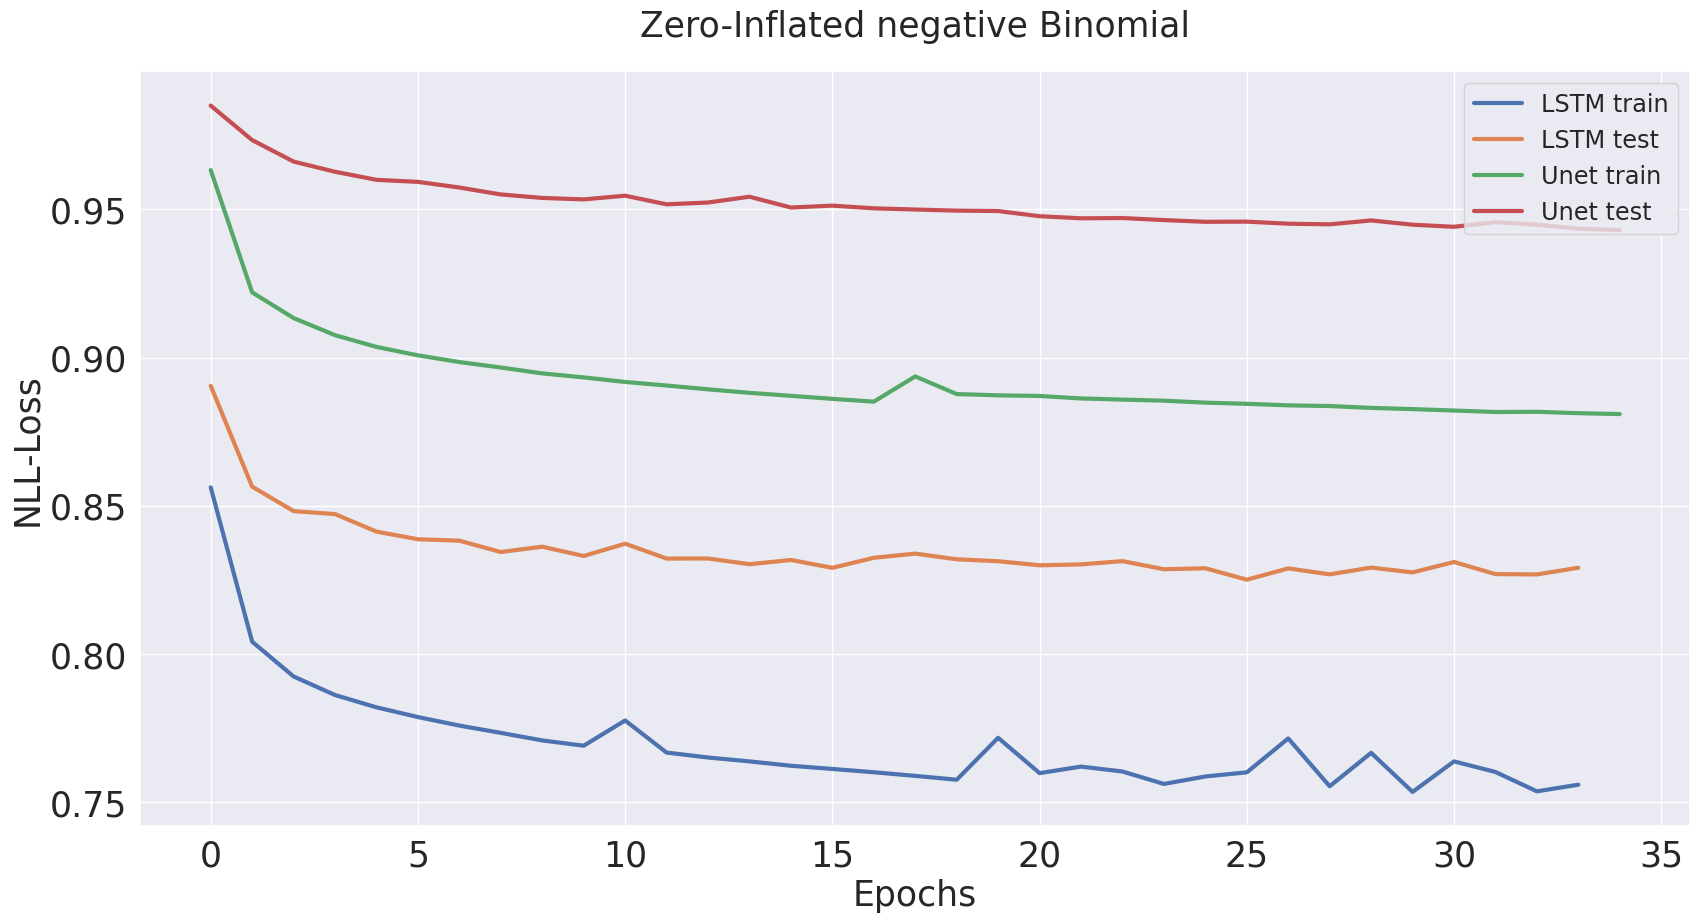
\includegraphics[width=0.9\textwidth,angle=0]{abb/Loss_zinfBinom.png}
 \caption{Trainingskurven für Zero-Inflated negativ Binomial verteilung}
\label{fig:Inception-Conv-LSTM}
\end{figure}

\noindent Zu sehen ist, dass die Unet-Architektur schlechtere Performance als die LSTM-Architektur liefert. In dieser Abbildung scheint der Overfitting bereich noch nicht erreicht worden zu sein.
Tatsächlich verbessern sich beide Architekturen noch marginal nach weiteren Epochen, aus Darstellungsgründen wurde die X-Achse auf 35 Epochen beschnitten.\\

\noindent Zusätzlich zur Zero-Inflated negative Binomial Verteilung wurden beide Architekturen mit einer weiteren Verteilung trainiert. Hierfür verwenden wir die Multinomiale Verteilung, woebei wir die Daten in Sieben Klassen einteilen. Die geschieht durch logarithmisches skalieren der Daten. Dadurch soll zusätzlich dem Klassenungleichgewicht entgegengesteuert werden (Regenwerte im höheren Bereich kommen seltener vor). 

\begin{figure}[htb]
 \centering
 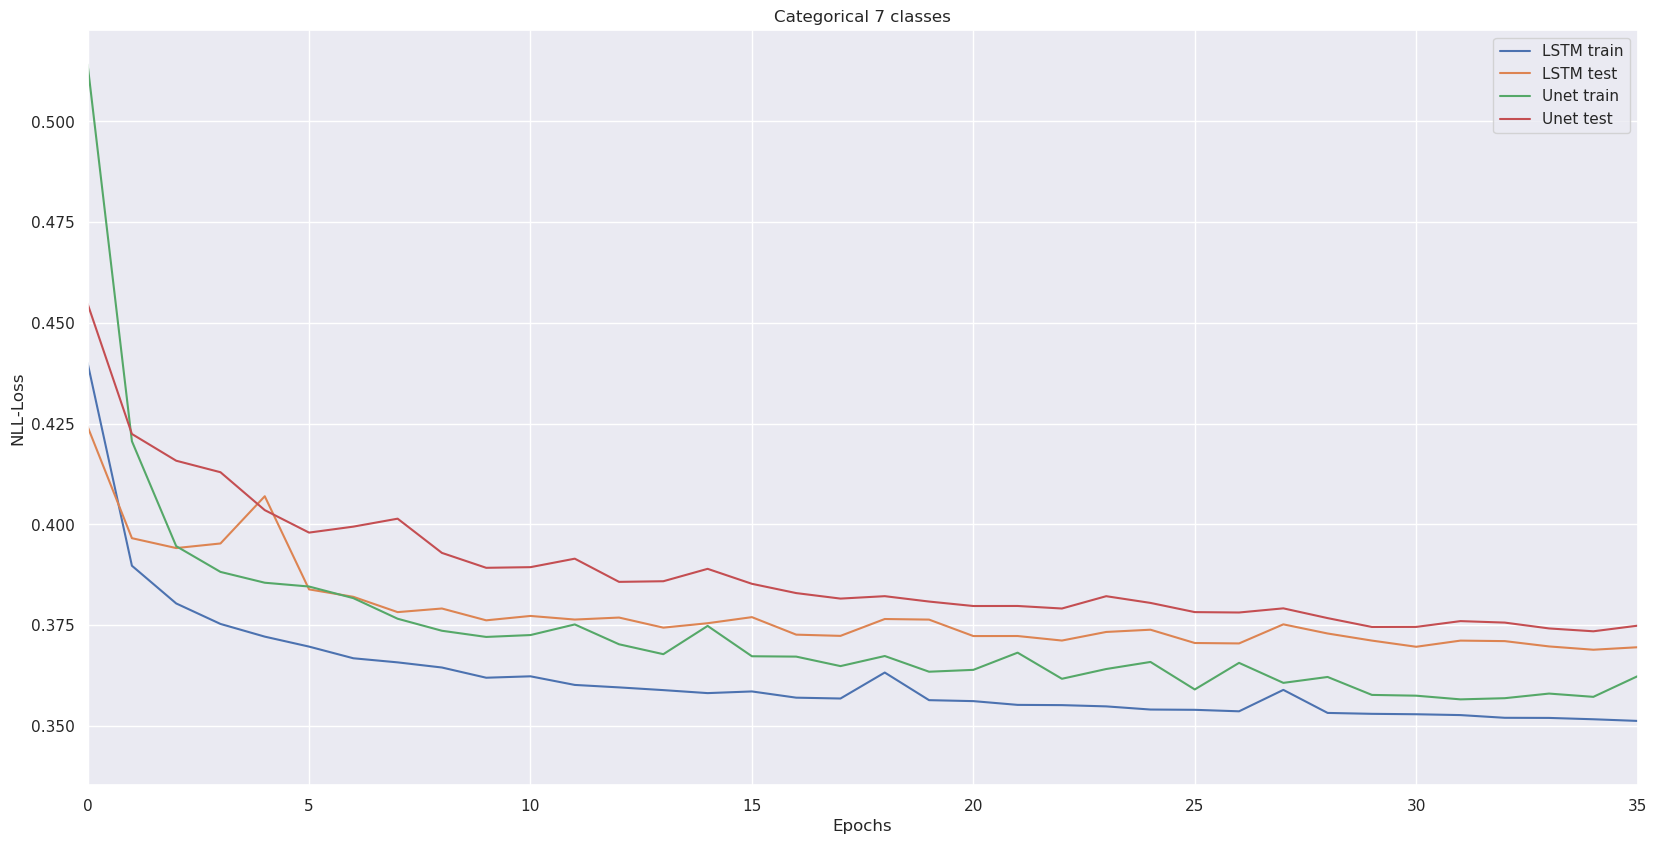
\includegraphics[width=0.9\textwidth,angle=0]{abb/Categorical.png}
 \caption{Multinomiale Verteilung}
\label{fig:multinomialeVerteilung}
\end{figure}

\noindent In der obigen Abbildung sind die Trainingskurven der beiden Architekturen zu sehen. Auch hier ist zu sehen, dass die LSTM-Architektur der Unet-Architektur überlegen ist und dies eine bessere Performance liefert. Vergleicht man die Trainingskurven für beide Verteilungen sieht man, dass der NLL für die Multinomiale Verteilung etwa die Hälfte der Zero-Inflated negative Binomialverteilung entspricht.

\newpage
\subsection{Auswertung}

Wir beschränken uns zuerst auf die Auswertung der binären Klassifikation von Regen und kein Regen. Später werden wir für die verschiedenen Architekturen und Verteilungen die Klassifikation für die Regenvorhersage begutachten.

\subsubsection{Baseline}
%TODO:

Die folgende Abbildung zeigt einen zufälligen Ausschnitt der Regenvorhersage für sieben aufeinanderfolgende Zeitschritte.\\

\begin{figure}[h]
\begin{tabular}{lllllll}
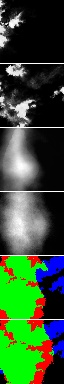
\includegraphics[width=20mm]{abb/prediction/100_maxCont}&
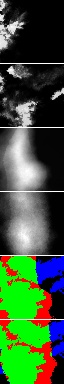
\includegraphics[width=20mm]{abb/prediction/101_maxCont}&
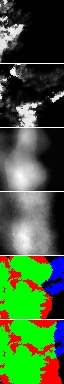
\includegraphics[width=20mm]{abb/prediction/102_maxCont}&
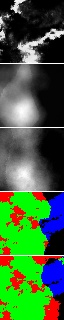
\includegraphics[width=20mm]{abb/prediction/103_maxCont}&
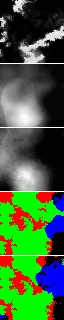
\includegraphics[width=20mm]{abb/prediction/104_maxCont}&
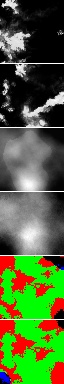
\includegraphics[width=20mm]{abb/prediction/105_maxCont}&
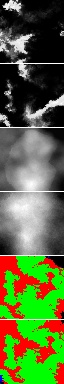
\includegraphics[width=20mm]{abb/prediction/106_maxCont}
\end{tabular}
\caption{Vorhersage in Abständen von fünf Minuten für die Zero-Inflated negative Binomialverteilung. Die erste Zeile entspricht dem momentanen Regen. Zeile zwei entspricht dem tatsächlichen Regen in 30 Minuten. Zeile drei ist die 30 Minuten Vorhersage des Unets. Zeile vier ist die 30 Minuten Vorhersage der LSTM-Architektur. Die Bilder sind kontrastmaximiert dargestellt. Die letzten beiden Zeilen stellen die korrekte bzw. inkorrekte Regenvorhersage für die Unet- und die LSTM-Architektur (letzte Zeile) dar.
Hierbei entspricht true positiv der Farbe Grün, false positiv Rot, false negativ Blau und true negativ Schwarz .\label{fig:predNegBin}}
\end{figure}

\noindent Anhand der Abbildung \ref{fig:predNegBin} ist zu sehen, dass für beide Architekturen tendenziell zu viel Regen vorhergesagt wird. Anhand der Bilder ist zudem zu sehen, dass Form der Regenfront nicht korrekt vorhergesagt wird. Des weiteren ist zu erkennen, dass false negativ (Blau) einen geringeren Teil der Vorhersage ausmachen. Durch die Kontrastmaximierte Darstellung der Vorhersage, sehen die Bilder so aus, als würden die maximalen Werte der Vorhersage in etwa der maximalen Werte des tatsächlichen Wetters entsprechen. Tatsächlich wird im allgemeinen die Regenmenge unterschätzt. Dies wird in einem späteren Teil der Auswertung dargelegt.\\



\begin{figure}[h]
\begin{tabular}{lllllll}
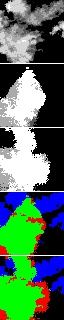
\includegraphics[width=20mm]{abb/prediction/100_cat_maxCont}&
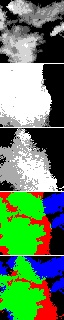
\includegraphics[width=20mm]{abb/prediction/101_cat_maxCont}&
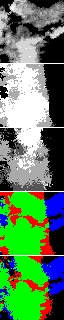
\includegraphics[width=20mm]{abb/prediction/102_cat_maxCont}&
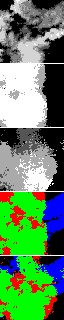
\includegraphics[width=20mm]{abb/prediction/103_cat_maxCont}&
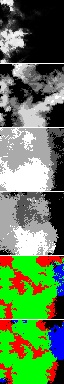
\includegraphics[width=20mm]{abb/prediction/104_cat_maxCont}&
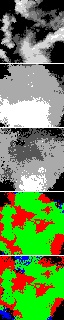
\includegraphics[width=20mm]{abb/prediction/105_cat_maxCont}&
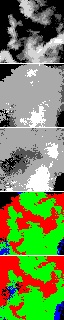
\includegraphics[width=20mm]{abb/prediction/106_cat_maxCont}
\end{tabular}
\caption{Vorhersage in Abständen von fünf Minuten für die Multinomialeverteilung. Hier sind die Zeilen wie in \ref{fig:predNegBin} dargestellt. Alle Bilder bis auf die Bilder der ersten Zeile sind in sieben Klassen dargestellt.\label{fig:predCat}}
\end{figure}


\noindent Auch bei der Multinomialenverteilung wird tendenziell zu viel Regen vorhergesagt.Des weiteren wird die Form der Regenfront nicht korrekt vorhergesagt. Zudem scheint die Anzahl der false negative (Blau) Vorhersagen höher als bei der Zero-Inflated negative Binomialverteilung. Zusammenfassend ist für die Ausschnitte der Vorhersagen zu sagen, dass die true positive vorhersagen die false negative und false positiv überwiegen. Um eine generelle Aussage treffen zu können wir im weiteren Verlauf die ''receiver operating characteristic'' auch \textbf{ROC} herangezogen.
\newpage

\noindent In der folgenden Abbildung ist die ROC für beide Architekturen und Verteilungen zu sehen. Die Kurven entstehen indem wir für verschiedene Schwellwerte die binäre Regenvorhersage treffen. Das bedeutet konkret, dass die Wahrscheinlichkeit für kein Regen berechnet wird. Ist diese Wahrscheinlichkeit größer als der Schwellwert so wird auch kein Regen vorhergesagt.
Die Schwellwerte liegen gleichmäßig verteilt zwischen Null und Eins.


\begin{figure}[h]
\begin{tabular}{cc}
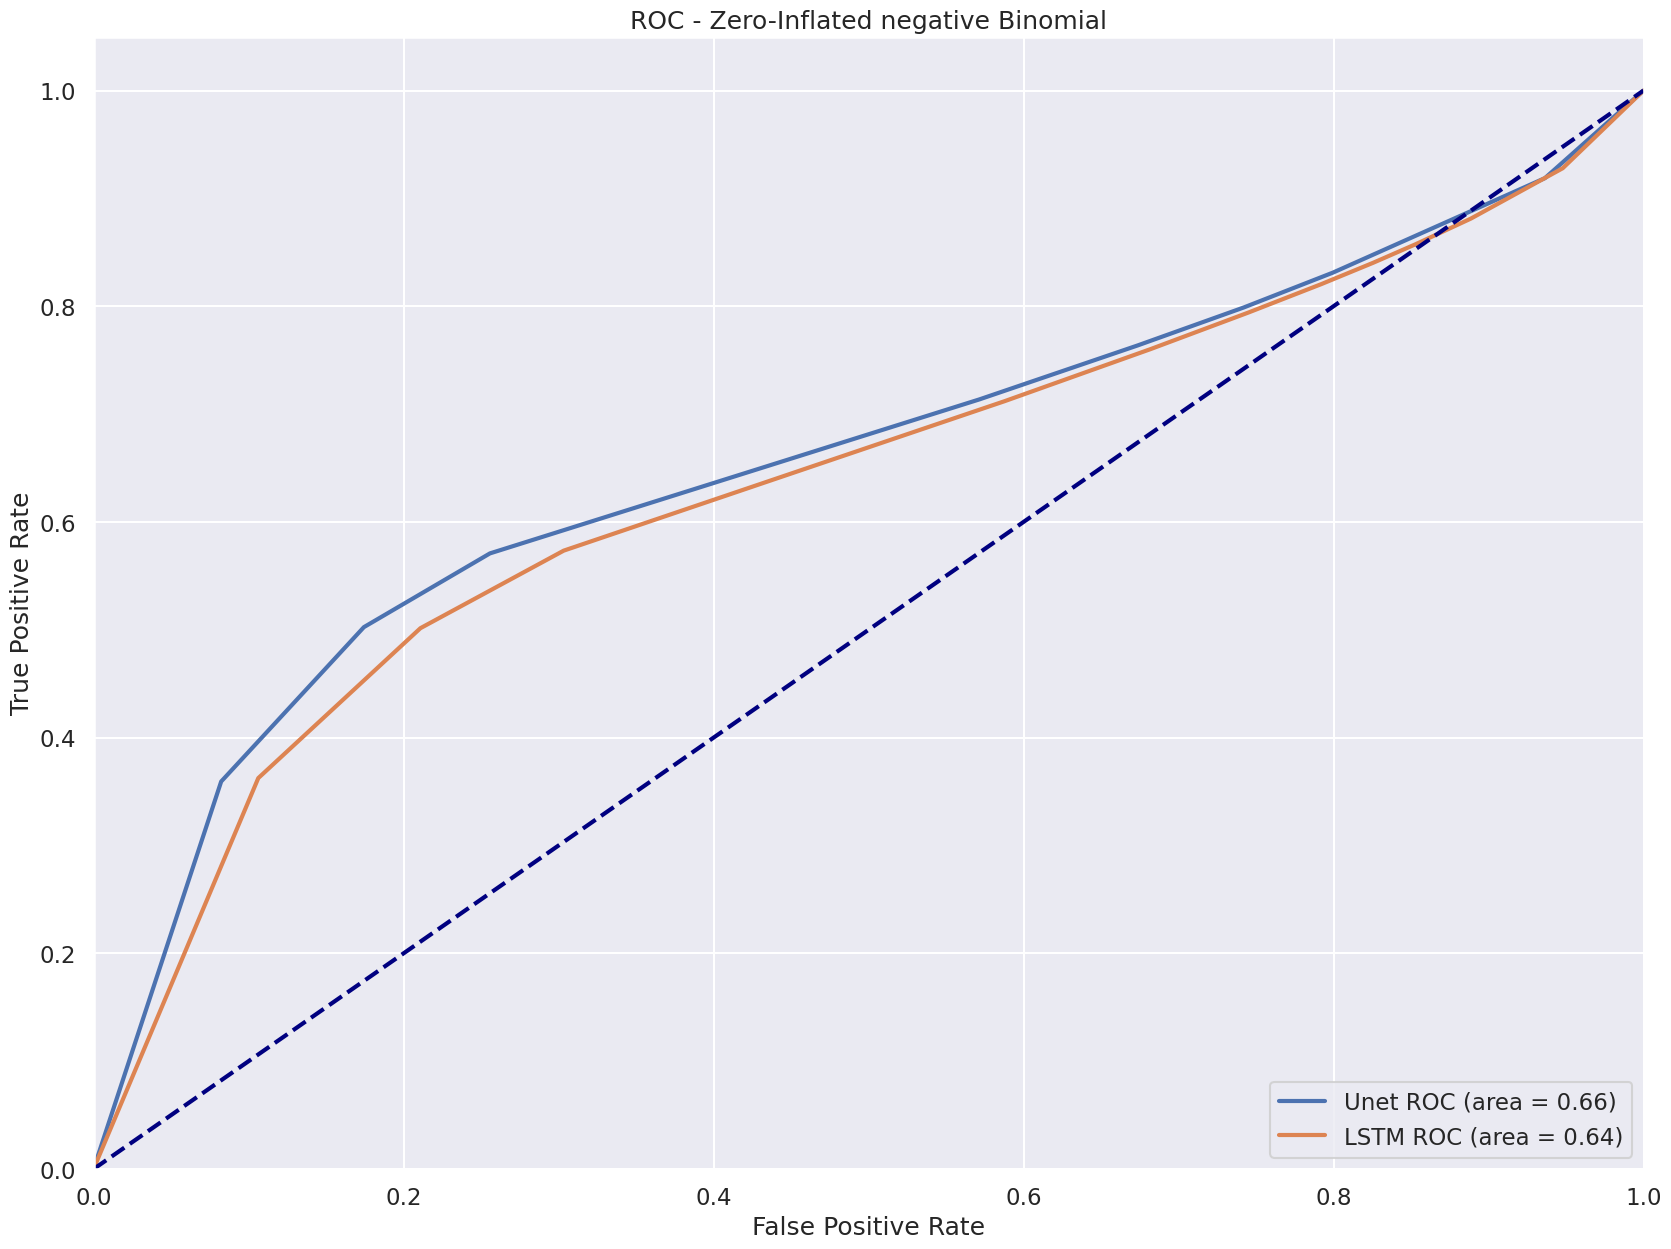
\includegraphics[width=70mm]{abb/ROC_ZINFBINOM.png}&
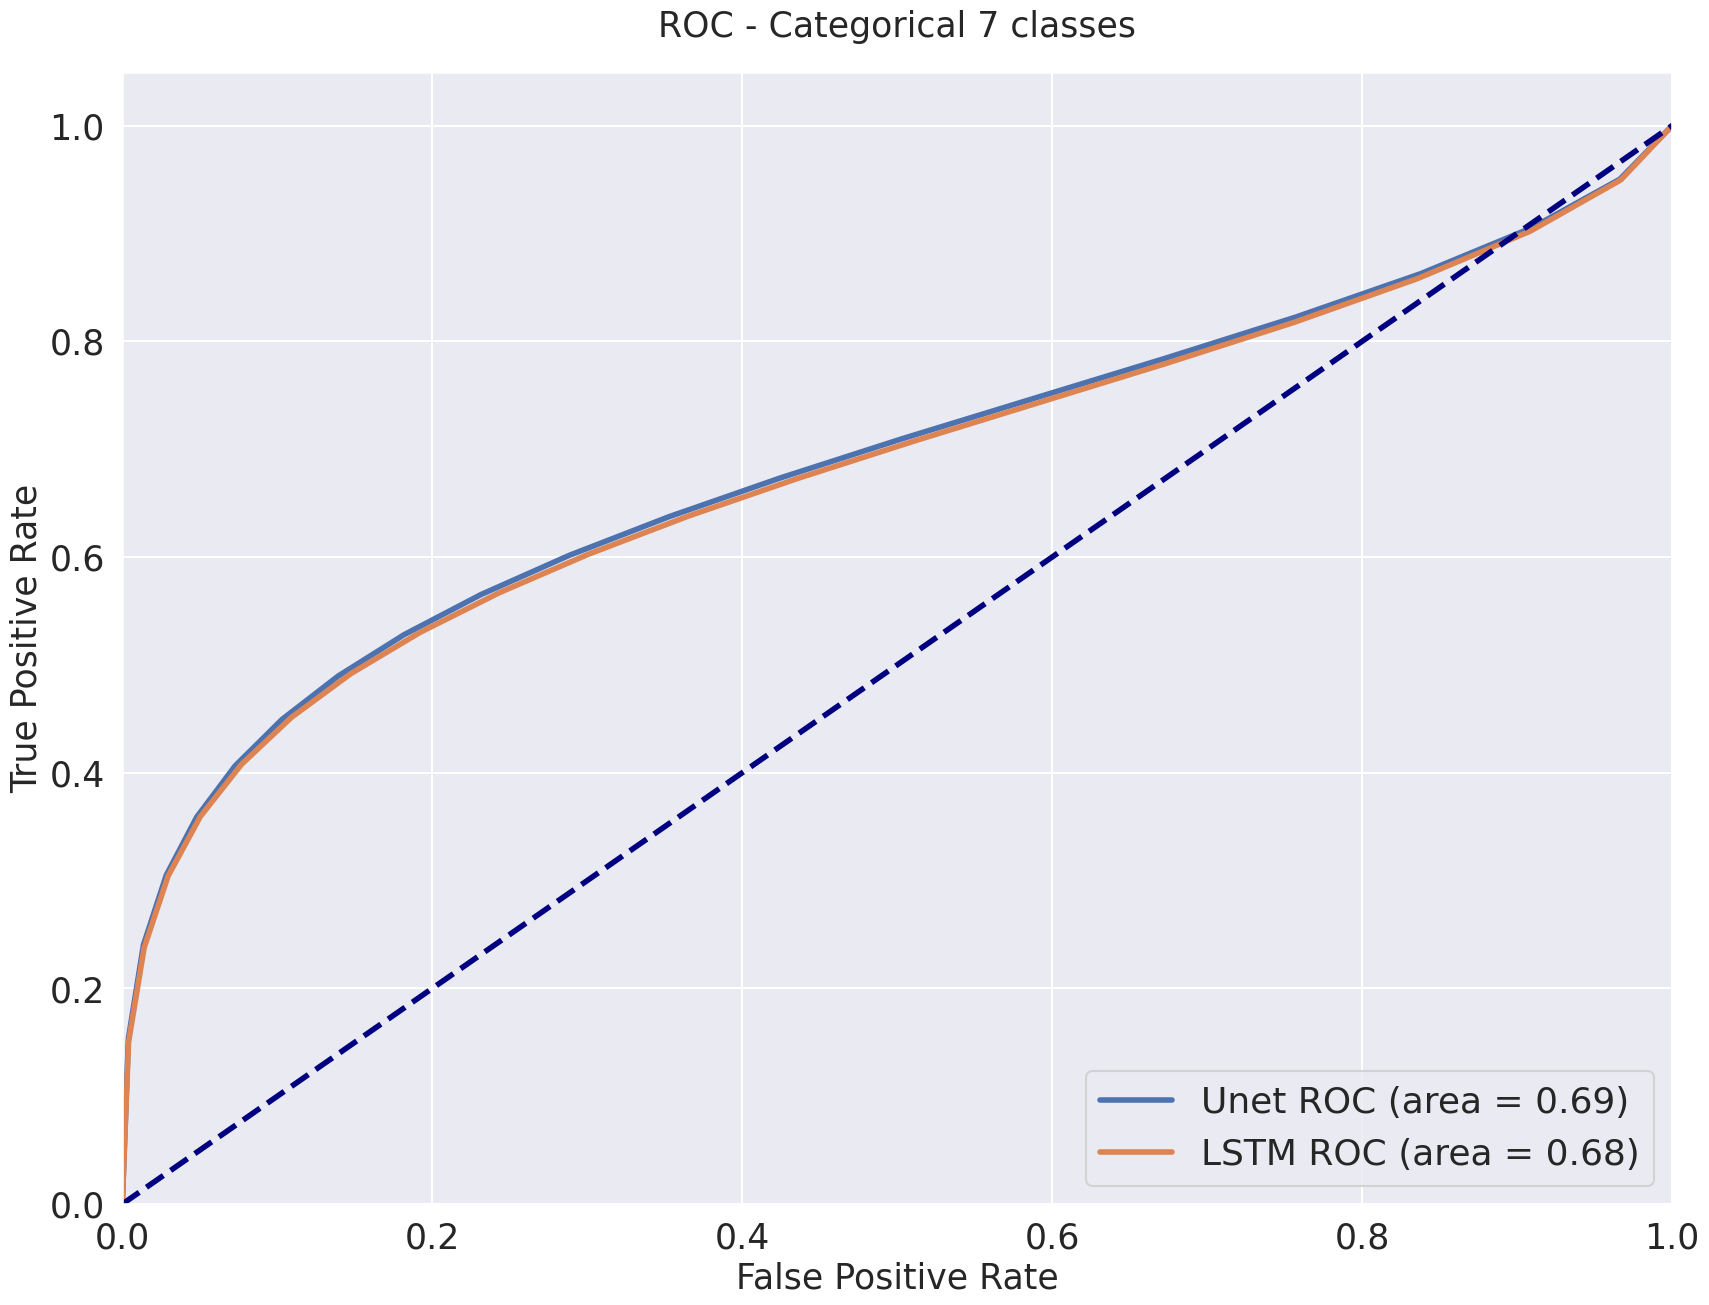
\includegraphics[width=70mm]{abb/ROC_Categorical.png}
\end{tabular}
\caption{ROC/AUR für beide Architekturen und beide Verteilungen. Links für die Zero-Inflated negativ Binomialverteilung und rechts für die Multinomialeverteilung.
Die Auserwertung erfolgt für 20 verschiedene Schwellwerte. \label{fig:anomerz}}
\end{figure}

\noindent Wie Anhand der Kurven zu erkennen ist, ist die ROC für die Multinomialeverteilung gleichmäßiger als die für die Zero-Inflated negativ Binomialverteilung. 
Auch die Fläche unter der Kurve (''area under curve'' \textbf{AUC}) ist für die Multinomialeverteilung marginal größer. Interessanterweise ist die Performance des Unets bei beiden Verteilungen besser (auch hier nur marginal) als für die LSTM-Architektur.\\

\noindent Für den Schwellwert 0.5 erhalten wir in beiden Fällen ein relativ gutes Verhältnis von true positiv zu false positiv. In den Nachfolgenden Abbildungen ist die Confusionmatrix für diesen Schwellwert zu sehen.



\begin{figure}[h]
\begin{tabular}{ccc}
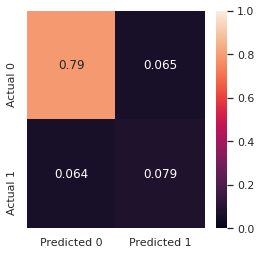
\includegraphics[width=45mm]{abb/simpleBaseLine.png}&
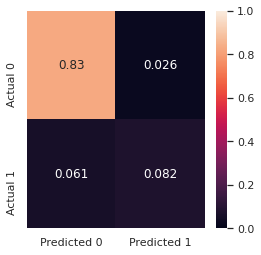
\includegraphics[width=45mm]{abb/znBinomConfusion_LSTM.png}&
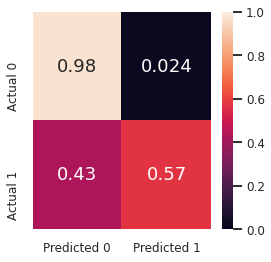
\includegraphics[width=45mm]{abb/znBinomConfusion_UNET.png}
\end{tabular}
\caption{Confusionmatrix für die Zero-Inflated negativ Binomialverteilung und dem Schwellwert 0.5. Links die einfache Baseline, mittig für die LSTM-Architektur und rechts für die Unet-Architektur. \label{fig:confusionmatrix_binom}}
\end{figure}

\noindent Anhand der Confusionmatrix ist zu sehen, dass die Netzwerke in beiden Fällen eine bessere Vorhersage liefern als die einfache Baseline. 
Anhand der Confusionmatrix wird das ungleichgewicht zwischen Regen und kein Regen deutlich. 

\begin{figure}[h]
\begin{tabular}{ccc}
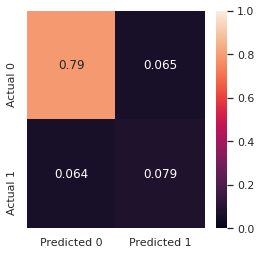
\includegraphics[width=45mm]{abb/simpleBaseLine.png}&
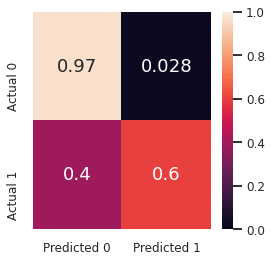
\includegraphics[width=45mm]{abb/categoricalConfusion_LSTM.png}&
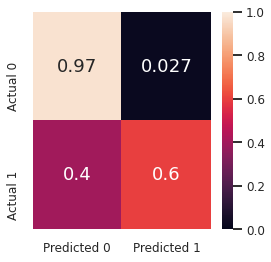
\includegraphics[width=45mm]{abb/categoricalConfusion_UNET.png}
\end{tabular}
\caption{Confusionmatrix für die Multinomialeverteilung und dem Schwellwert 0.5. Links die einfache Baseline, mittig für die LSTM-Architektur und rechts für die Unet-Architektur. \label{fig:confusionmatrix_cat}}
\end{figure}

\noindent Auch für die Multinomialeverteilung erhalten wir eine bessere Vorhersage als mit der einfachen Baseline.
Vergleichen wir die Confusionmatrix beider Verteilungen, so lässt sich feststellen, dass die Verteilungen in verschiedenen Bereichen andere Vorteile aufweisen.
So ist die Regenvorhersage für die Multinomialeverteilung etwas besser als für die Zero-Inflated negativ Binomialverteilung. Letztere (insbesondere die Unet-Variante) produziert mehr true negative und weniger false positiv Vorhersagen als die Multinomialeverteilung.\\

\noindent Für die tatsächliche Regenvorhersage ist jedoch interessant, in wie vielen Fällen eine Person Nass wird obwohl kein Regen vorhergesagt wird.
Dazu wird die untere Zeile der Confusionmatrix mit einem Faktor multipliziert, sodass deren Summe 100 ergibt.\\
\begin{table}[h]
\begin{tabular}[h]{l|c|c}
Verteilung & Person wird Nass & Person wird nicht Nass  \\
\hline
Multinomialeverteilung & \textbf{39,9} \% & \textbf{60,1} \%  \\
Zero-Inflated negativ Binomialverteilung &43,0 \% & 57,0 \%  \\
Einfache Baseline & 44,8 \% & 55,2 \% 
\end{tabular}
\caption{\label{tab:nass}}
\end{table}

\noindent Aus der Tabelle \ref{tab:nass} hervorgeht, wird die Person die sich auf die Vorhersage verlässt mit einer Wahrscheinlichkeit von 39,1 (im besten Fall) \% Nass.
Dies ist zwar nicht überragend, es ist jedoch besser als würde sich die Person darauf verlassen, dass das Wetter so bleibt wie es ist.



\newpage


\section{Die DeepRainApp und das Datenbankhandling}\label{die deeprain app und das datenbankhandling}
In den folgenden Abschnitten werden alle Komponenten behandelt welche benötigt werden um die Vorhersage Daten in der DeepRain App anzuzeigen und die volle Funktionalität der App zu gewährleisten.  

\subsection{Übersicht}\label{übersicht}
Die Komponente “App und Datenbankhandling” besteht zum wesentlich aus diese drei Unterkomponenten.  

\begin{figure}[h]
 \centering
 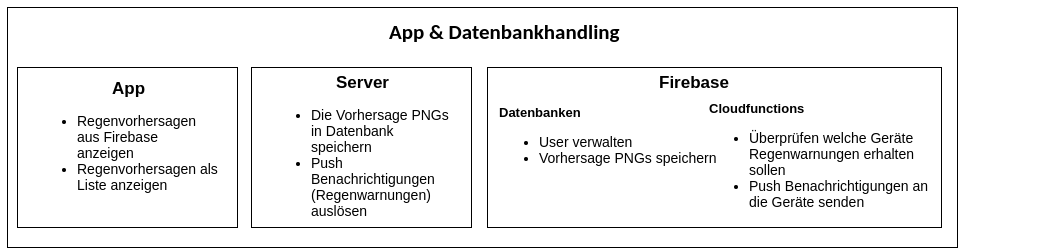
\includegraphics[width=1\textwidth,angle=0]{abb/app_datenbank_komponente_uebersicht}
 \caption[Komponentenübersicht App und Datenbankhandling]{Die Komponente App und Datenbankhandling}
\label{fig:Beschreibung}
\end{figure}

Die App dient zur Visualisierung der Daten und macht somit die Regenvorhersagen für den Endnutzer brauchbar. 
Auf dem Server werden die Vorhersagen berechnet und in dem für dieses Kapitel relevanten Teil
für die App zur Verfügung gestellt. 
Die Firebase verbindet den Server mit der App und erfüllt dabei im wesentlichen zwei verschiedene Aufgaben. 
Sie stellt die Regenvorhersagen als PNG für die App zur Verfügung und übernimmt das  Senden der Pushbenachrichtigungen,
welche für die Regenwarnungen gebraucht werden.
 

\subsection{Firebase}\label{firebase}
Firebase ist eine Entwicklungsplattform für mobile Apps. 
Diese stellt verschiedene Services zur Verfügung, welche es ermöglichen, effizient Apps für IOS und Android zu entwickeln. 
Die Firebase ist ein zentraler Baustein der Komponente und wird in jeder Unterkomponente verwendet, weshalb hier einführend 
ein Überblick gegeben werden soll. 
Firebase stellt eine Datenbank und einen Cloud-Speicher zur Verfügung, welcher genutzt wird, um die User zu verwalten und die 
Vorhersage PNGs auf den Geräten anzuzeigen.
Des Weiteren werden die In-App Messaging Dienste von Firebase verwendet, um die Regenwarnungen in Form von Push Benachrichtigungen zu senden. 
Die genaue Funktionsweise wird in dem Kapitel “Push Nachrichten” beschrieben.   
Firebase ist bis zu einem gewissen Punkt der Verwendung komplett kostenlos. 
Wird dieser Punkt überschritten, sind die Kosten von der tatsächlichen Nutzung abhängig. 
In der kostenlosen Version enthalten sind 1 GB Cloud-Speicher, von welchem aktuell nur ein Bruchteil für die 20 PNGs 
verwendet wird. Des Weiteren können am Tag bis zu 20.000 Dokumente geschrieben und 125.000 Dokumente gelesen werden. 
Durch die komplett überarbeitete Datenbank und Softwarearchitektur wurden die Datenbanknutzung so weit verringert, 
dass diese Limitierungen bei Weitem nicht erreicht werden sollten.
\subsection{Datenbank und Cloudspeicher}\label{datenbank und cloudspeicher}
Die verwendete Datenbank ist ein Firestore von Firebase. Firestore ist ein Cloud NOSQL Datenbanksystem. 
Die Daten werden in sogenannte Kollektionen und Dokumente eingeteilt. 
Dabei gehören zu jeder Kollektion Dokumente, in welchen die eigentlichen Daten gespeichert sind. 
In Abbildung \ref{fig:datenbank_aufbau} ist der Datenbankaufbau zu sehen.
\begin{figure}[h]
 \centering
 \includegraphics[width=0.6\textwidth,angle=0]{abb/datenbank_aufbau_übersicht}
 \caption[Datenbankarchitektur]{Der Aufbau der Kollektionen und Dokumente in der Firebase}
\label{fig:datenbank_aufbau}
\end{figure}

Jedes Gerät besitzt einen einmaligen Device Token welcher in zwei Kollektionen gespeichert wird. 
Die Eine Kollektion steht für den Zeitpunkt in dem die Regenwarnung gesendet werden soll, die andere Kollektion steht für die Region in der die App verwendet wird. 
Diese beiden Kollektionen werden für das Senden der Push Benachrichtigungen benötigt, in dem Kapitel \ref{sec:Pushbenachrichtigungen} wird darauf genauer eingegangen. 
In den Einstellungen der App kann eingestellt werden wann die Regenwarnung als Push-Benachrichtigung gesendet werden soll.
Je nachdem was der User einstellt, wird sein Devicetoken in eine andere Kollektion gespeichert. 
Dabei gibt es für jede einstellbare Zeit ein eigenes Dokument in der Kollektion TimeBeforeWarning. 
Wenn die Netze Regen vorhersagen wird vom Server ein Dokument in RainWarningPushNotification gepusht. 
Dieses Dokument wird von einer Cloud-Function (Siehe Kapitel \ref{sec:Pushbenachrichtigungen}) verwendet um die Push Benachrichtigungen an die richtigen Geräte zu senden.
Der Cloud Storage von Firebase wird verwendet um die PNGs mit der jeweiligen Vorhersage zu speichern.
Dabei pushed der Server alle 5 Minuten die neuen Vorhersagen. Diese PNGs werden in der App angezeigt. 
\subsection{Server}\label{server}
Mit der Serverkomponente ist der Teil des Servers gemeint, der für die Kommunikation mit der Firebase verantwortlich ist. Dazu gehört das bereitstellen der aktuellsten Regendaten in Zahlen und Bildformat sowie das triggern von Push Benachrichtigungen. 
Da zu beginn des Projektes noch keine Vorhersagen von den Netzen zur Verfügung stand, wurde ein Programm entwickelt, dass den Server simuliert und zufällig generierte Regendaten in der Firebase speichert. Somit konnte die App unabhängig und parallel zu den Netzen entwickelt werden. 
Für alle vorhandenen Regionen in denen Device Tokens gespeichert sind, es also Nutzer in der Region gibt, wird über den jeweiligen Breiten und Höhengrad der dazugehörige Pixel für die Region berechnet.
Wenn der Server ein Vorhersage PNG bekommt, bei dem die Regenstärke über einem bestimmten Grenzwert liegt, wird ein Dokument in der Kollektion RainWarningPushNotification gespeichert, welches von der Cloud Funktion verwendet wird, um eine Regenwarnung an die Geräte zu schicken. 
\subsection{Die App}\label{die app}

\subsubsection{Funktionen der App}\label{funkionen der app}
Die App soll die von den Netzen berechnete Vorhersagen visualisieren und dem Benutzer zur Verfügung stellen. Die Daten werden dabei sowohl in 
Tabellarischer als auch in Form einer Karte dargestellt. Dabei wird gewährleistet, dass immer die aktuellsten Daten zur Verfügung stehen. 
Außerdem wird der Benutzer benachrichtigt, sobald es eine Regenwarnung gibt. Der Zeitpunkt der Regenwarnung kann eingestellt werden.
Für Präsentationszwecke wurde der Demo Modus eingeführt. In diesem werden Beispiel Vorhersage Daten angezeigt.

\subsubsection{Screens der App}\label{screens der app}
Im Wesentlichen besteht die App aus drei Screens. Einem Screen zum Anzeigen der Daten in Listenform, 
einem zum Anzeigen der Daten auf einer Karte und den Einstellungen. 
Die jeweiligen Screens können über die Bottomnavigation erreicht werden, somit ist es möglich, intuitiv zwischen den einzelnen 
Screens zu wechseln.
Im Folgenden wird auf die einzelnen Screens und deren technische Funktionsweise genauer eingegangen.
\begin{figure}[H]
    \centering
    \subfloat[][]{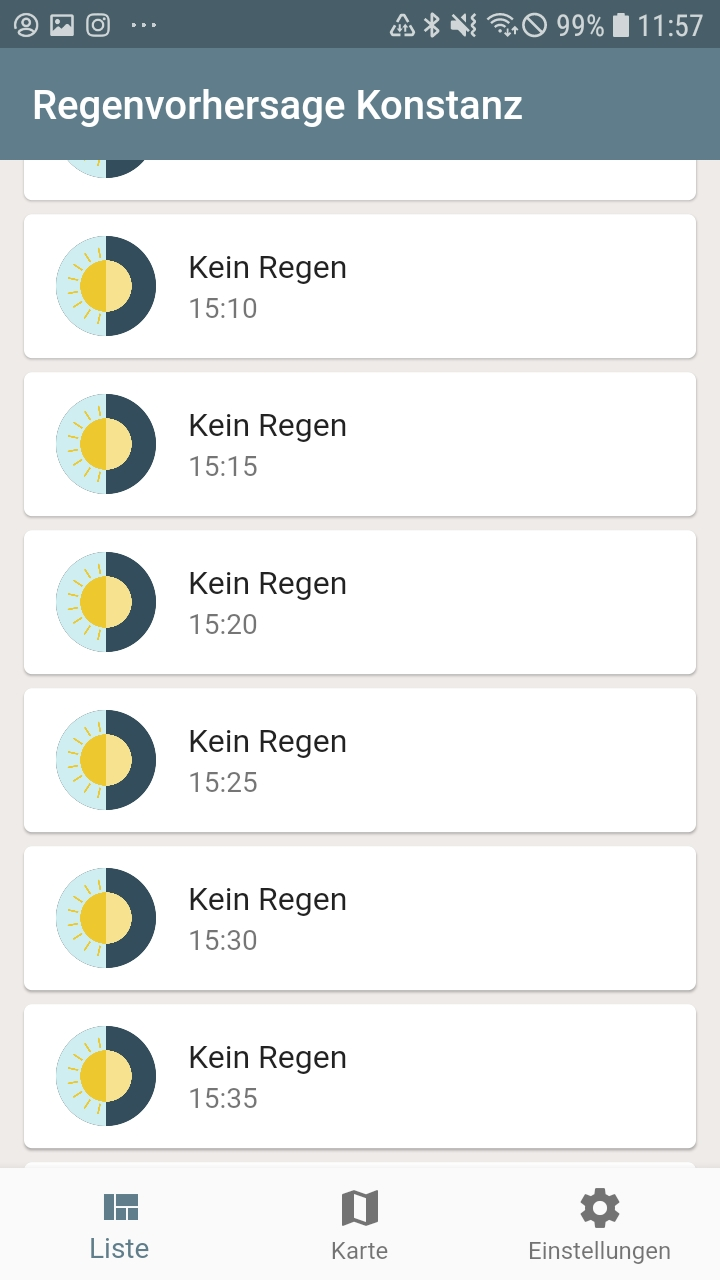
\includegraphics[width=0.3\linewidth]{abb/screenshot_forecast_list}}
    \subfloat[][]{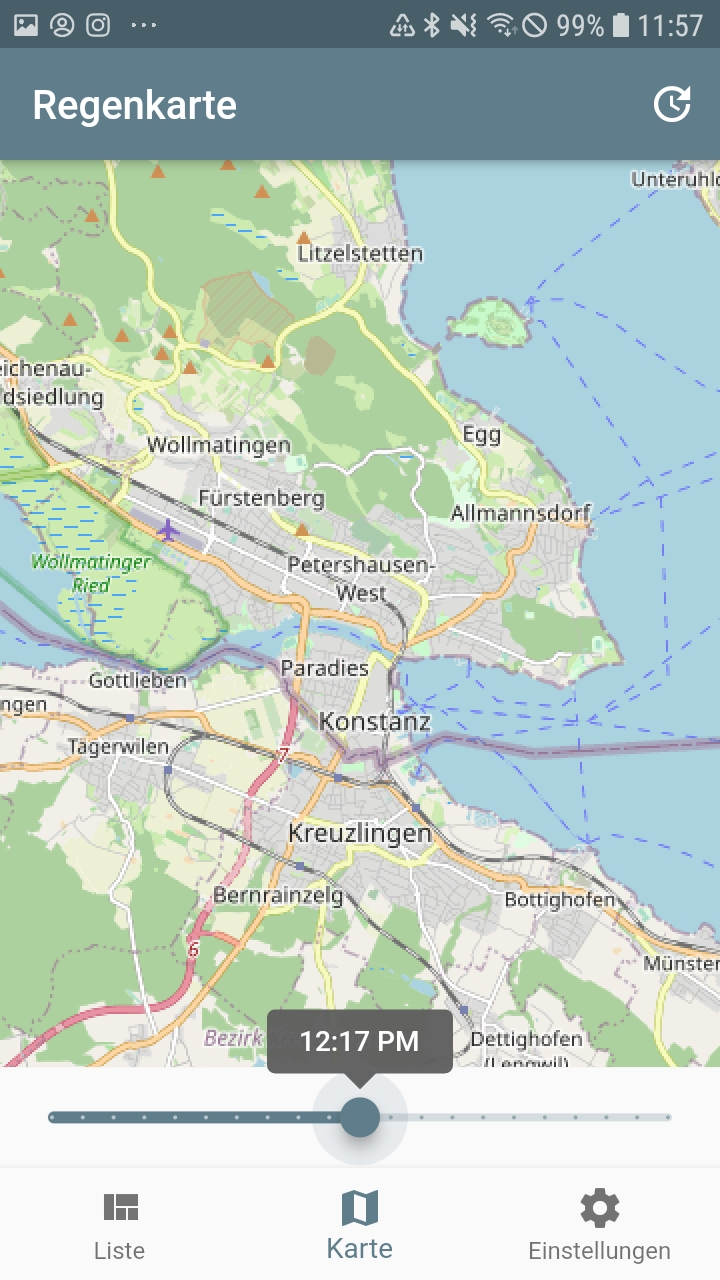
\includegraphics[width=0.3\linewidth]{abb/screenshot_forecast_map}}
    \subfloat[][]{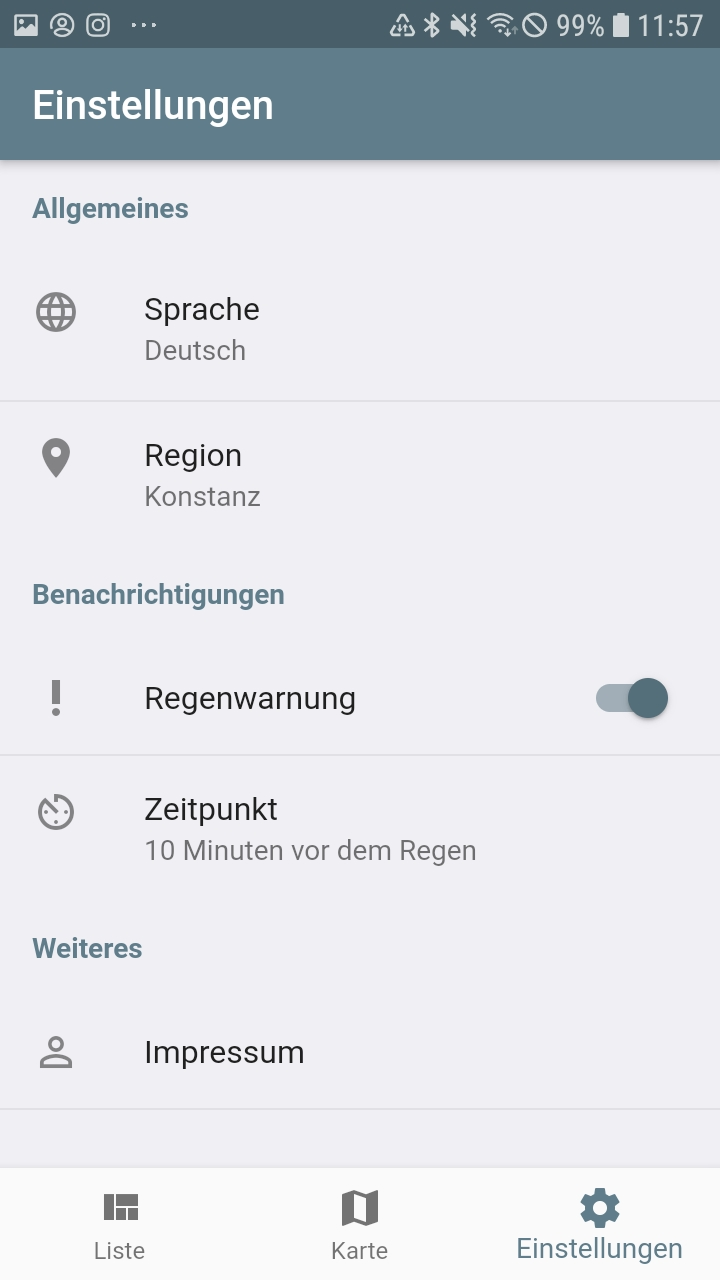
\includegraphics[width=0.3\linewidth]{abb/screenshot_settings}}
    \caption{Die drei Hauptscreens der App}
\end{figure}

\subsubsection*{Regenvorhersage als Liste}
Auf diesem Screen werden die von den Netzen berechneten Regenvorhersagen angezeigt. 
Dabei wird in die drei Kategorien “Kein Regen”, “Leichter Regen” und “Starker Regen” unterschieden. 
Je höher die berechnete Regenintensität ist, je dunkler wird der Regenschirm, welcher zu Beginn jedes einzelnen Listeneintrages zu sehen ist.   
Die anzuzeigenden Daten werden während dem Appstart in der Klasse ProvideForecastData gespeichert und können währende der Laufzeit
von dort gelesen werden.

\subsubsection*{Regenvorhersage als Karte}
Auf diesem Screen werden die von den Netzen erzeugten PNGs visualisiert. 
Dafür werden die PNGs mit einer Karte hinterlegt, auf welcher der User frei navigieren kann, 
um die aktuelle Regensituation an jedem beliebigen Ort zu prüfen. 
Dabei wird standardmäßig der Kartenausschnitt von der Region angezeigt, die in den Einstellungen eingestellt wurde. 
Mit dem Slider kann der Zeitpunkt eingestellt werden, in dem die Regenvorhersage angezeigt werden soll. 
Mit dem Aktualisieren Button in der Actionbar können die neusten Bilder vom Server heruntergeladen werden. 
Aufgrund der verhältnismäßig großen Datenmenge werden die neuen Vorhersagen nicht automatisch vom Server heruntergeladen. 
Im Normalfall werden die Bilder einmalig bei dem App Start heruntergeladen.

\subsubsection*{Einstellungen}
Auf diesem Screen können alle relevanten Einstellungen gemacht werden. Dazu gehört z.B. die Sprache der Benutzeroberfläche. 
Außerdem kann die Region eingestellt werden. 
Die hier ausgewählte Region wird standardmäßig auf der Karte angezeigt und nur für diese Region werden Regenwarnungen gesendet. 
Unter der Benachrichtigungs Kategorie können die Regenwarnungen aktiviert und der Zeitpunkt der Regenwarnung eingestellt werden. 
Jede Aktion in dieser Kategorie löst verschiedene Datenbankaufrufe aus. 
Wenn die Regenwarnung aktiviert wird, wird der Devicetoken von dem Gerät in die Datenbank hochgeladen, beim Deaktivieren wird der Devicetoken gelöscht. 
Wenn der Zeitpunkt der Regenwarnung verändert wird, wird der Devicetoken in der Datenbank von einer Kollektion in eine andere Kollektion verschoben.   
Alle gemachten Einstellungen werden in sogenannten Shared Preferences gespeichert, damit sie auch nach Appstart noch vorhanden sind.   
In Abbildung \ref*{fig:sequence_diagram_change_settings} ist der Datenfluss beim Anpassen des Zeitpunktes für die Regenwarnung 
dargestellt. 

\begin{figure}[H]
 \centering
 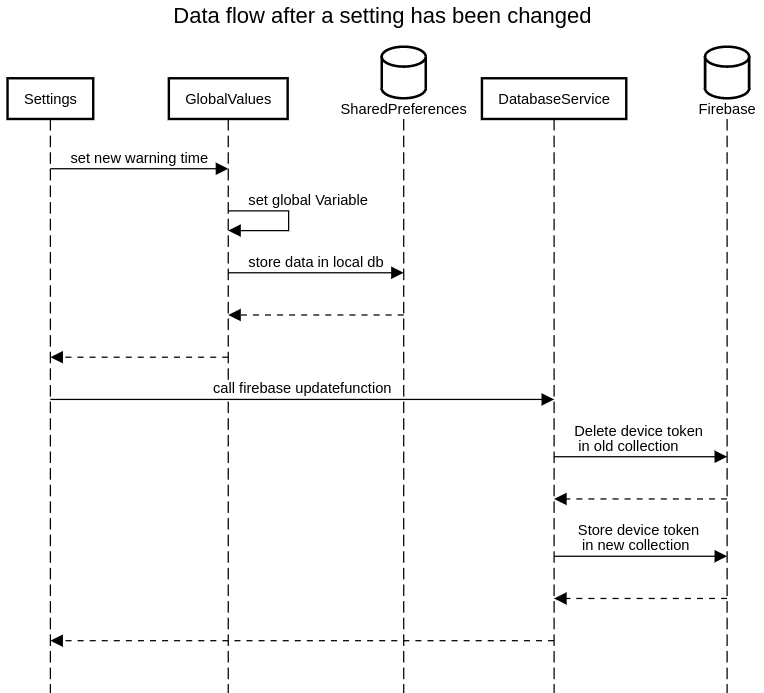
\includegraphics[width=0.8\textwidth,angle=0]{abb/sequence_diagram_change_settings}
 \caption[Sequencediagram Einstellungen ändern]{Der Datenfluss beim ändern des Zeitpunktes der Regenwarnung}
\label{fig:sequence_diagram_change_settings}
\end{figure}

\subsubsection{Der Appstart}
Während dem Appstart wird die App für die Verwendung vorbereitet, Einstellungen werden wieder hergestellt und
die aktuellen Regenvorhersagen werden aus der Datenbank heruntergeladen. 
Die Einstellungen können dabei aus den Shared Preferences ausgelesen werden. 
Die Shared Preferences sind eine lokale Key-Value Datenbank, in der alle benutzerspezifischen Daten gespeichert werden. 
Bei dem App Start werden die Einstellungen aus den Shared Preferences gelesen und auf globale Variablen gespeichert, somit
sind sie während der Laufzeit der App dynamisch verfügbar. 
Außerdem wird bei dem ersten Appstart die Position in dem Vorhersagebild berechnet. 
Diese wird benötigt, um aus den Vorhersagebildern den richtigen Pixel auszulesen und in der Vorhersageliste anzuzeigen.
Der Appstart ist in folgender Abbildung schematisch dargestellt.

\begin{figure}[H]
 \centering
 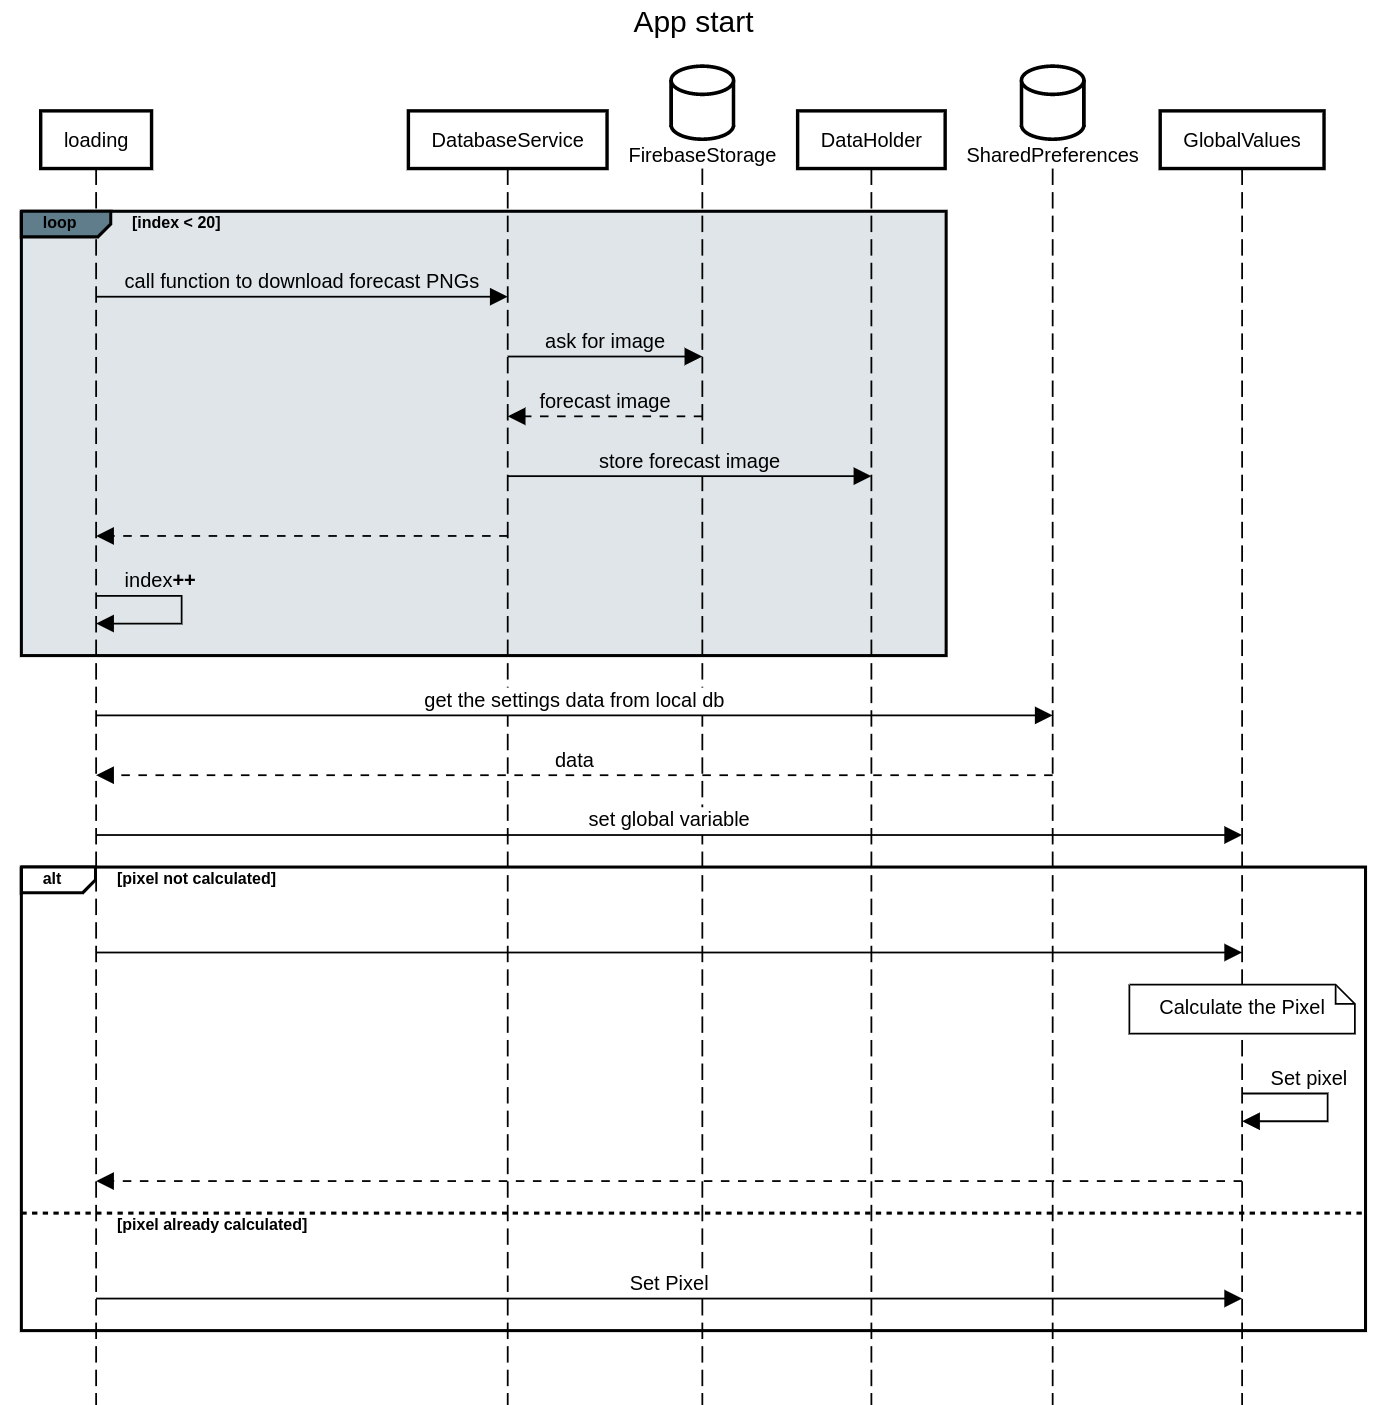
\includegraphics[width=0.8\textwidth,angle=0]{abb/sequence_diagram_app_start}
 \caption[Sequencediagram Appstart]{Datenfluss beim starten der App inklusive der Datenbankabfragen (Server und Lokale Datenbank)}
\label{fig:sequence_diagram_app_start}
\end{figure}

\subsubsection{Die Berechnung der Regenintensität}
Zu Beginn wurde angenommen, dass die App nur in Konstanz verwendet werden soll. 
Im Laufe des Projektes stellte sich jedoch heraus, dass die entwickelten Netze in der Lage sind, Vorhersagen 
für ganz Deutschland zu machen. Da die Softwarearchitektur nicht für eine solche Anwendung ausgelegt war, 
mussten einige Änderungen vorgenommen werden. 
Bis zu diesem Zeitpunkt wurden die Vorhersage Daten für jeden Pixel auf dem Server berechnet und im Anschluss in 
der Firebase gespeichert. 
Bei verschiedenen Nutzern in verschiedenen Regionen kommt diese Architektur allerdings schnell an seine Grenzen. 
Hat die App bspw. 1000 Nutzer in verschiedenen Regionen, 
müssen für jeden der 1000 Nutzer alle fünf Minuten 20 Vorhersage Daten hochgeladen werden. 
Daher musste der Datenfluss so umstrukturiert werden, dass der neue Regenwert direkt in der App berechnet wird. 
Dabei muss das Handy den entsprechenden, eigenen Pixel auf der Karte berechnen. 
Die Berechnung hierfür ist verhältnismäßig aufwendig, da mit großen Listen (810.000 Einträge) gearbeitet werden muss.
Auf diese Berechnung wird in Abschnitt \ref{sec: pixel_berechnung} eingegangen. 

Wenn die Bilder beim Appstart oder bei einem Vorhersageupdate heruntergeladen werden, wird von jedem Bild der Regenwert 
in dem entsprechenden Pixel berechnet. 
Es wird eine Liste mit ForecastListItem Objekten erstellt. Diese wird global gespeichert und in der Vorhersage Liste angezeigt. 
Aktuell können nur beim App Start oder durch manuelles Auslösen eines Updates die Vorhersage Daten aktualisiert werden.  

\subsubsection{Berechnung des Pixels} \label{sec: pixel_berechnung}
Um die Regensituation an dem jeweiligen Ort des Users auszuwerten, muss der Pixel in dem Vorhersagebild berechnet werden. 
Hierfür dienen drei verschiedene Listen. Diese Listen wurden in Python mit der Wradlib erstellt, und anschließend 
im JSON Format in die App übertragen. 
Zwei der Listen enthalten alle Latitude bzw. Longitude Werte.
Die Koordinaten in den einzelnen Indizes kombiniert geben die Position der einzelnen Pixel im Weltkoordinatensystem an.
In der dritten Liste steht zu jedem Index die jeweilig zugehörige Pixel Koordinate im Bild. 
Somit steht jeder Index für eine Position im Weltkoordinatensystem, ausgedrückt durch Höhen und Breitengrad Informationen
und der Abbildung dieser Position auf den Vorhersagebild.
Da das Bild eine Auflösung von 900x900 Pixeln hat, sind diese Listen 810.000 Elemente groß.
\begin{figure}[H]
  \centering
  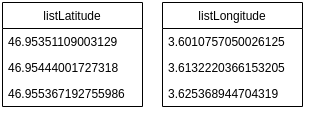
\includegraphics[width=0.8\textwidth,angle=0]{abb/listen_pixel_berechnung.png}
  \caption{Der Exemplarische Aufbau der Listen zur Berechnung des eigenen Pixels}
 \label{fig:sequence_diagram_app_start}
 \end{figure}
 Jeder User hat eine eigene Position in Deutschland, welche in Form von Höhen und Breitengrad angaben bekannt ist. 
 Diese wird durch die in den Einstellungen festgelegte Region bestimmt. 
 Es wird nun also ein Algorithmus gesucht, der mithilfe der Höhen und Breitengrad Informationen den Pixel im Bild findet, 
 der am besten zu diesen Koordinaten passt. 
 Nun wäre es natürlich möglich, durch alle Indizes zu Iterieren und somit den richtigen Pixel zu finden. Dieses Verfahren 
 ist aber sehr Zeit und rechenintensiv und daher nicht geeignet um es auf einem Smartphone auszuführen.

 Wir brauchen noch eine Lösung!! 

\subsubsection{Framework Entscheidung}\label{framework entscheidung}
Bei der Entwicklung einer App steht die Frage der zu bedienenden Plattformen an erster Stelle. Soll die App zum Beispiel nur unternehmensintern verwendet 
werden oder ist das Gerät auf dem sie verwendet wird eine Neuanschaffung kann es ausreichend sein nativ auf einer Plattform zu entwickeln. Soll jedoch, 
wie bei den meisten Apps, eine breite Zielgruppe angesprochen werden, ist es unerlässlich, die App auf IOS und Android zur Verfügung zu stellen. 
je nachdem, auf welchen Betriebssystemen die App verwendet werden soll, muss eine komplett andere Frameworkwahl getroffen werden. 
So würde man, wenn man entweder nur für IOS oder Android entwickeln möchte, zu einer der nativen Lösungen greifen. Je nach Anforderungen kann auch, 
wenn beide Betriebssysteme bedient werden sollen, zu der nativen Lösung gegriffen werden. In dem Fall muss der komplette Code doppelt 
geschrieben werden. Daher wird normalerweise auf Frameworks zurückgegriffen, welche beide Betriebssysteme bedienen. 
Einige bekannte Frameworks sind zum Beispiel Xamarin, React Native oder Flutter. Jedes dieser Frameworks ist zukunftsträchtig und wurde von großen 
Unternehmen auf den Markt gebracht. So steht Microsoft hinter Xamarin, Facebook hinter React Native und Google hinter Flutter. 
Je nach Frameworkwahl kann von ca. 80-100 Prozent von dem kompletten Code für beide Betriebssysteme verwendet werden. 
Dafür sind Cross-Plattform Frameworks oft nicht so performant wie die nativen. Dies fällt besonders bei rechenaufwendigen Apps und Spielen ins Gewicht. 
Bei so einer leichten App wie DeepRain fällt dieser Nachteil nicht ins Gewicht. Außerdem hätten wir auch nicht genug Kapazitäten um zwei native und 
voneinander unabhängige Apps zu entwickeln. 
Ein großer Vorteil von Flutter ist, dass 100 Prozent der Codebasis für Android und IOS übernommen werden können. Außerdem hat die Prominenz von 
Flutter in den letzten Jahren seit der Veröffentlichung stark zugenommen. In der folgenden Abbildung sind die Google Suchanfragen für den Begriff 
Flutter abgebildet.  Das in Kombination mit eigenem Interesse an dem Framework, ist der Grund dafür, dass die DeepRain App mit Flutter entwickelt wurde.
\begin{figure}[H]
 \centering
 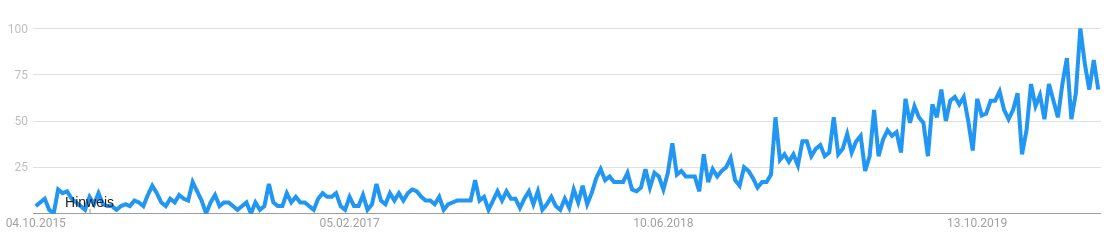
\includegraphics[width=0.8\textwidth,angle=0]{abb/flutter_google_trends}
 \caption[Entwicklung von Flutter]{Entwicklung der Suchanfragen für den Begriff 'Flutter'}
\label{fig:flutter_google_trends}
\end{figure}

\subsubsection{Technischer Aufbau von Flutter}
Flutter Anwendungen werden in der Programmiersprache Dart geschrieben und können anschließend für IOS, Android, Windows, Linux, MacOs und als WebApp 
veröffentlicht werden. Dart bringt dabei im Vergleich zu Java Script den Vorteil mit, dass es objektorientiert ist, was vor allem in größeren 
Softwarearchitekturen zum tragen kommt. Auch alle Bibliotheken um Code asynchron auszuführen, werden bereits von Dart mitgeliefert. 
Die wohl größte Rolle für jeden Dart Entwickler spielen die sogenannten Widgets. Widgets sind einzelne Bausteine, welche die UI repräsentieren. 
Jedes UI Element ist dabei ein eigenes Widget. Dabei werden Widgets oft ineinander geschachtelt, was es ermöglicht, komplexere UI’s zu entwerfen. 
Dabei werden Widgets in Stateless und Statefull Widgets unterschieden. Während ein Stateless Widget keine Daten und somit keinen Zustand speichern kann, 
ist das mit einem Stateful Widget möglich.

Die Grundlage von Flutter sind Widgets. \\
Wie funktioniert flutter?   \\
Was ist der Unterschied zu anderen hybriden Frameworks?  \\ 
Nur eine Codebasis \\
Keine weiteren Frameworks nötig\\
Alles dabei, UI, Widgets, Animationen\\

\subsubsection{Projektstruktur}
Der gesamte Code der App ist in die fünf Ordner DataObjects, global, screens, services und Widgets aufgeteilt. 
Die erste verwendete Datei ist main.dart. In dieser wird festgelegt welcher Screen als erstes nach dem Start 
aufgerufen wird und die Bottom Navigation wird konfiguriert. 
Für jeden Screen der App gibt es eine .dart datei in dem Ordner Screens. 
Welche Files gibt es? \\
Welche Klassen gibt es? \\
Wie arbeitet was zusammen? \\
\begin{figure}[H]
  \centering
  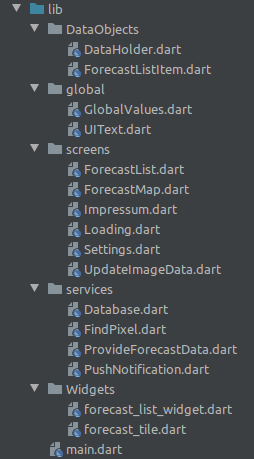
\includegraphics[width=0.3\textwidth,angle=0]{abb/projektstruktur}
  \caption{Die Projektstruktur der App}
 \label{fig:projektstruktur_app}
 \end{figure}

\subsection{Cloudfunktionen}
Mit den Cloudfunktionen von Firebase kann Backend-Code direkt auf den Servern von Google gespeichert und ausgeführt werden. 
Dabei ist es möglich, auf bestimmte Datenbankaktionen zu reagieren. 
Diese Funktionalität wird verwendet, um Push Benachrichtigungen zu senden. 
Der Code wird in Java Script geschrieben und anschließend als Cloud Funktion hochgeladen.

\subsubsection{Push Benachrichtigungen}\label{sec:Pushbenachrichtigungen}
Zum Warnen der Benutzer, wenn es eine Regenvorhersage gibt, werden Push Nachrichten verwendet. 
Der Zeitpunkt der Push Benachrichtigungen kann in der App eingestellt werden. 
So kann man sich zwischen 5 und 60 Minuten vor dem bevorstehenden Regen warnen lassen.  
Um eine Pushbenachrichtigung zu versenden, speichert der Server ein Dokument in der Firebase welches alle für die 
Pushbenachrichtigung relevanten Informationen enthält. 
Dazu gehört zum Beispiel der Push Benachrichtigungstitel und Text, sowie die Zeit bis der Regen eintritt.
Sobald das neue Dokument mit den Informationen für die Push Benachrichtigung hochgeladen wurde, wird eine Callback 
Funktion in Form einer Cloudfunktion aufgerufen.
Je nachdem, zu welchem Zeitpunkt ein User die Regenwarnung erhalten möchte, wird sein Device Token in eine andere 
Kollektion gespeichert.   
Außerdem wird je nach Region, in der sich der User befindet, sein Token in einer anderen Kollektion gespeichert. 
Nur die Tokens, die sowohl mit dem Zeitpunkt, als auch mit der Region, aus dem vom Server hochgeladenen Dokument übereinstimmen, 
sollen eine Pushbenachrichtigung erhalten. 
Die Funktion findet diese Schnittmenge und weiß somit, welche Geräte eine Pushbenachrichtigung erhalten sollen.

\begin{figure}[H]
 \centering
 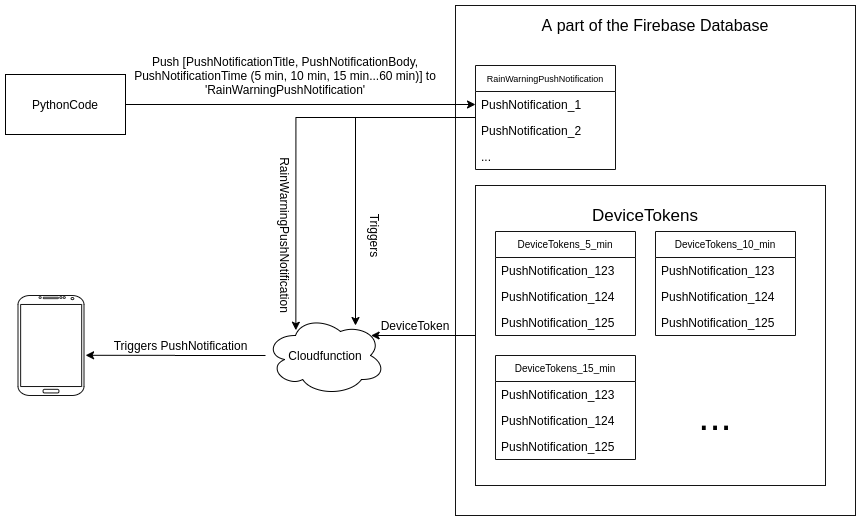
\includegraphics[width=0.8\textwidth,angle=0]{abb/funktionsweise_pushnachrichten_senden}
 \caption[Funktionsweise von Pushbenachrichtigungen]{Funktionsweise des Prozesses zum senden von Push - Benachrichtigungen.}
\label{fig:funktionsweise_pushnachrichten_senden}
\end{figure}

\subsection{Vorgehen bei Entwicklung}
In Flutter entwickelte Apps können sowohl auf Android als auch auf IOS ausgeführt werden. 
Um eine Flutter App auf einem IPhone auszuführen, wird allerdings MacOS als Betriebssystem benötigt. 
Da während des Entwicklungsprozesses nur ein Linuxrechner zur Verfügung stand, wurde die App lange Zeit nur unter
Android getestet. 
Erst gegen Ende des Projektes wurde der Code für IOS kompiliert und für das IPhone angepasst.  
Da die gesamte Pipeline zu beginn noch nicht funktioniert hat, wurde der für die App relevante Teil der Pipeline simuliert.
Dazu wurde ein Pythonprogramm geschrieben, welches reale Daten in die Firebase pushed. 
Somit war es möglich, gekapselt vom Rest des Projektes zu arbeiten und die App fertigzustellen.


    



\section{Pipeline}\label{sec: Pipeline}
Nachdem die einzelnen Komponenten für sich funktionieren gilt es sie in einer Pipeline zu kombinieren und so ein funktionierendes Gesamtkonzept zu erhalten.
Der dadurch entstehende Workflow lässt sich in die Bereiche Datenbeschaffung, Regenvorhersage sowie Datenaufbereitung und Bereitstellung aufteilen.
Diese werden im Folgenden erläutert.

\subsection{Datenbeschaffung}
Zum Training sowie zur Validierung der Netze konnten bisher historische Daten verwendet werden.
Um eine Praxistaugliche Wettervorersage zu berechnen, muss diese allerdings in der Zukunft liegen.
Die Input Daten der Netze müssen daher möglichst aktuell sein.
Hiefür wurden, wie bereits bei den Historischen Daten, Daten des DWDs genutzt.
Dieser stellt alle fünf Minuten aktuelle Binärradardaten bereit.
Das Skript prüft alle fünf Sekunden ob neue Daten bereit stehen, falls das der Fall ist, werden diese heruntergeladen und anschließend wie in Abschnitt \ref{die datenaufbereitung} erläutert in Bilder mit einer Auflösung von 900x900 Pixeln konvertiert.
Anschließend wird ein Auschnitt des Bildes genommen welcher gegebenenfalls skaliert werden kann.
So kann der Ort für die Spätere Wettervorersage leicht angepasst werden.

\subsection{Regenvorhersage}
Die Vorhersage selbst hängt stark von den eingesetzten Netzen ab.
Derzeit werden drei gleiche Netze eingesetz welche auf 10, 20 und 30 Minuten vorhersagen trainert wurden.
Als Input für jedes Netz werden die 5 aktuellsten Bilder verwendet.
Deren Werte werden normiert und anschließend in einen Batch mit der Shape (1, 96, 96, 5) gebracht.

\subsection{Datenaufbereitung und Bereitstellung}
Die berechnete Vorhersage hat einen Wertebereich von 0-255 und eine Auflösung von 64x64 Pixel.
Um die Vorhersage in der App richtig darstellen zu können muss diese noch weiter bearbeitet werden.
Um vorhersagen flexibel an verschiedenen Orten oder in verschiedenen Auflösungen bereitstellen zu können ohne die App anzupassen, stellt diese für jede Vorhersage ein PNG mit 900x900 Pixeln dar.
Daher muss der Ausschnitt mit der Vorhersage bzw. mit den historischen Daten an der richtigen Position des PNGs eingefügt werden.
Die Pixel außerhalb dieses Auschnitts sind transparent.
Die unterschiedlichen Regenstärken werden mit drei verschiedenen Blautönen dargestellt.
Da die Regenintensität wie in Abschnitt \ref{die datenaufbereitung} erläutert nicht gleichverteilt ist, wurden die Schwellwerte zwei und zehn gewählt. 
Zudem wird jedem historischen Bild sowie jeder Vorhersage eine Zeitpunkt zugewiesen welcher später auf dem Slider in der App visualisiert wird.
Nun können die fünf historischen Regenbilder sowie die drei Vorhersagen in der Firebase-Datenbank ersetzt und so der App, also dem Nutzer bereitgestellt werden. 
Der Vorgang wiederholt sich und es wird alle fünf Sekunden geprüft ob auf dem Server des DWDs neue Daten vorhanden sind. 



\section{Ausblick}
Entzerrung der Vorhersage Bilder\\
Optimierung der Netzte\\
Netzte die mehr als ein Zeitschritt vorhersagen?\\


\section{Fazit}
Mit DeepRain wurde ein Grundbaustein gelegt, auf dessen Basis in Zukunft aufgebaut werden kann. 
Es wurde ein komplett funktionsfähiges Gesamtsystem entwickelt, dass die Daten vom Server des DWD bis an den User bringt.
Es wurde eine App entwickelt die alle Anforderungen erfüllt und stabil funktioniert. 
Es ist mit minimalem Aufwand möglich, zukünftige Netze in das Gesamtsystem und die App zu integrieren. 
Um das Gesamtsystem praxistauglich zu machen, müssen die Netze weiterentwickelt werden. 
Durch das miterleben eines Projektes dieses Umfangs, konnten wir viel lernen. 
Durch die breit gefächerten Aufgabengebiete war es uns möglich in viele verschiedene Themengebiete einen Einblick zu erhalten. 
Gleichzeitig konnte sich jedes Teammitglied einen eigenen Schwerpunkt setzten, in dem es besonders tief in die Materie einsteigen konnte. 
Nur durch die gute Teamarbeit und Koordination war es möglich, ein Projekt dieser Größe umzusetzen. 


\noindent Wir persönlich sind mit dem Endergebnis mehr als zufrieden und hoffen, dass das Projekt erfolgreich weitergeführt wird.




% In dieser Datei ist viel Beispielcode für alle möglichen Arten von Formattierungen usw.
%% einzelne Kapitel werden hier eingebunden
\section{Einleitung}\label{einleitung}

Hier steht die Einleitung der Arbeit... Lorem ipsum dolor sit amet, consetetur sadipscing elitr, sed diam nonumy eirmod tempor invidunt ut labore et dolore magna aliquyam erat, sed diam voluptua. At vero eos et accusam et justo duo dolores et ea rebum. Stet clita kasd gubergren, no sea takimata sanctus est Lorem ipsum dolor sit amet. Lorem ipsum dolor sit amet, consetetur sadipscing elitr, sed diam nonumy eirmod tempor invidunt ut labore et dolore magna aliquyam erat, sed diam voluptua. At vero eos et accusam et justo duo dolores et ea rebum. Stet clita kasd gubergren, no sea takimata sanctus est Lorem ipsum dolor sit amet.

\newpage

\section{Hauptabschnitt}\label{hauptabschnitt}

Text des ersten Abschnitts... Lorem ipsum dolor sit amet, consetetur sadipscing elitr, sed diam nonumy eirmod tempor invidunt ut labore et dolore magna aliquyam erat, sed diam voluptua. At vero eos et accusam et justo duo dolores et ea rebum. Stet clita kasd gubergren, no sea takimata sanctus est Lorem ipsum dolor sit amet. Lorem ipsum dolor sit amet, consetetur sadipscing elitr, sed diam nonumy eirmod tempor invidunt ut labore et dolore magna aliquyam erat, sed diam voluptua. At vero eos et accusam et justo duo dolores et ea rebum. Stet clita kasd gubergren, no sea takimata sanctus est Lorem ipsum dolor sit amet.

\subsection{Unterabschnitt 1}\label{unterabschnitt_1}

Erstes Unterabschnitt

\subsection{Unterabschnitt 2}\label{unterabschnitt_2}

Zweites Unterabschnitt

\subsection{Unterabschnitt 3}\label{unterabschnitt_3}

Drittes Unterabschnitt

\newpage

\section{Weiterer Hauptabschnitt}\label{hauptabschnitt_2}

Text des zweiten Abschnitts... Lorem ipsum dolor sit amet, consetetur sadipscing elitr, sed diam nonumy eirmod tempor invidunt ut labore et dolore magna aliquyam erat, sed diam voluptua. At vero eos et accusam et justo duo dolores et ea rebum. Stet clita kasd gubergren, no sea takimata sanctus est Lorem ipsum dolor sit amet. Lorem ipsum dolor sit amet, consetetur sadipscing elitr, sed diam nonumy eirmod tempor invidunt ut labore et dolore magna aliquyam erat, sed diam voluptua. At vero eos et accusam et justo duo dolores et ea rebum. Stet clita kasd gubergren, no sea takimata sanctus est Lorem ipsum dolor sit amet.

\newpage

% hier können weitere Kapitel angelegt und eingetragen werden
% ....

\section{Ausblick}\label{ausblick}

Text des Ausblicks - sofern dies in der Arbeit gewünscht ist... Lorem ipsum dolor sit amet, consetetur sadipscing elitr, sed diam nonumy eirmod tempor invidunt ut labore et dolore magna aliquyam erat, sed diam voluptua. At vero eos et accusam et justo duo dolores et ea rebum. Stet clita kasd gubergren, no sea takimata sanctus est Lorem ipsum dolor sit amet. Lorem ipsum dolor sit amet, consetetur sadipscing elitr, sed diam nonumy eirmod tempor invidunt ut labore et dolore magna aliquyam erat, sed diam voluptua. At vero eos et accusam et justo duo dolores et ea rebum. Stet clita kasd gubergren, no sea takimata sanctus est Lorem ipsum dolor sit amet.

\newpage

\section{Fazit}\label{fazit}

Text des Fazits... Lorem ipsum dolor sit amet, consetetur sadipscing elitr, sed diam nonumy eirmod tempor invidunt ut labore et dolore magna aliquyam erat, sed diam voluptua. At vero eos et accusam et justo duo dolores et ea rebum. Stet clita kasd gubergren, no sea takimata sanctus est Lorem ipsum dolor sit amet. Lorem ipsum dolor sit amet, consetetur sadipscing elitr, sed diam nonumy eirmod tempor invidunt ut labore et dolore magna aliquyam erat, sed diam voluptua. At vero eos et accusam et justo duo dolores et ea rebum. Stet clita kasd gubergren, no sea takimata sanctus est Lorem ipsum dolor sit amet.


% Beispiel für Bild mit Fußnote
\begin{figure}[htb]
 \centering
 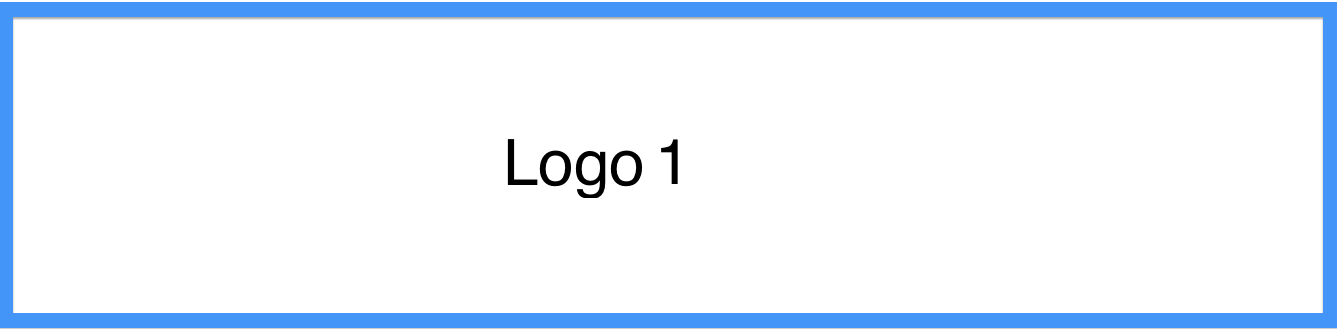
\includegraphics[width=0.4\textwidth,angle=45]{abb/logo1}
 \caption[Beispiel einer Bildbeschreibung]{Beispiel einer Bildbeschreibung\footnotemark}
\label{fig:beispiel1}
\end{figure}
\footnotetext{Bildquelle: Beispiel einer Bildquelle}

% Beispiel für Bildintegration
\begin{figure}[htb]
 \centering
 \includegraphics[width=0.3\textwidth,angle=0]{abb/logo2}
 \caption[Beschreibung]{Beschreibung}
\label{fig:Beschreibung}
\end{figure}

% Beispiel: Referenz auf Abbildung
Abbildung~\ref{fig:Beschreibung} [S.\pageref{fig:Beschreibung}]

% Beispiel: Tabelle 
\begin{center}
  \begin{tabular}{ | l | c | }
    \hline
    Überschrift 1 & Überschrift 2 \\ \hline \hline
    Info 1 & Info 2 \\ \hline
    Info 3 & Info 4 \\ \hline
    \hline
    \multicolumn{2}{|c|}{Info in einer Zelle} \\
    \hline
  \end{tabular}
\end{center}


% Beispiel für Quellcode Listings
\lstset{language=xml}
\begin{lstlisting}[frame=htrbl, caption={Die Datei {\normalfont \ttfamily  data-config.xml} dient als Beispiel für XML Quellcode}, label={lst:dataconfigxml}]
<dataConfig>
  <dataSource type="JdbcDataSource" 
              driver="com.mysql.jdbc.Driver"
              url="jdbc:mysql://localhost/bms_db"
              user="root" 
              password=""/>
  <document>
    <entity name="id"
        query="select id, htmlBody, sentDate, sentFrom, subject, textBody
        from mail">
    <field column="id" name="id"/>
    <field column="htmlBody" name="text"/>
    <field column="sentDate" name="sentDate"/>
    <field column="sentFrom" name="sentFrom"/>
    <field column="subject"  name="subject"/>
    <field column="textBody" name="text"/>
    </entity>
  </document>
</dataConfig>
\end{lstlisting}

\lstset{language=java}
\begin{lstlisting}[frame=htrbl, caption={Das Listing zeigt Java Quellcode}, label={lst:result2}]
/* generate TagCloud */
Cloud cloud = new Cloud();
cloud.setMaxWeight(_maxSizeOfText);
cloud.setMinWeight(_minSizeOfText);
cloud.setTagCase(Case.LOWER);
	    
/* evaluate context and find additional stopwords */
String query = getContextQuery(_context);
List<String> contextStoplist = new ArrayList<String>();
contextStoplist = getStopwordsFromDB(query);
	    
/* append context stoplist */
while(contextStoplist != null && !contextStoplist.isEmpty())
  _stoplist.add(contextStoplist.remove(0));
	    
/* add cloud filters */
if (_stoplist != null) {
  DictionaryFilter df = new DictionaryFilter(_stoplist);
  cloud.addInputFilter(df);
}
/* remove empty tags */
NonNullFilter<Tag> nnf = new NonNullFilter<Tag>();
cloud.addInputFilter(nnf);

/* set minimum tag length */
MinLengthFilter mlf = new MinLengthFilter(_minTagLength);
cloud.addInputFilter(mlf);

/* add taglist to tagcloud */
cloud.addText(_taglist);

/* set number of shown tags */	    
cloud.setMaxTagsToDisplay(_tagsToDisplay);
\end{lstlisting}


% Beispiel für Formeln
Die Zuordnung aller möglichen Werte, welche eine Zufallsvariable annehmen kann nennt man \emph{Verteilungsfunktion} von $X$.

\begin{quotation}
Die Funktion F: $\mathbb{R} \rightarrow$ [0,1] mit $F(t) = P (X \le t)$ heißt Verteilungsfunktion von $X$.\footnote{Mustermann, vgl.~\cite{mm2009}~[S.55]}
\end{quotation}

\begin{quotation}
Für eine stetige Zufallsvariable $X: \Omega \rightarrow \mathbb{R}$ heißt eine integrierbare, nichtnegative reelle Funktion $w: \mathbb{R} \rightarrow \mathbb{R}$ mit $F(x) = P(X \le x) = \int_{-\infty}^{x} w(t)dt$ die \emph{Dichte} oder \emph{Wahrscheinlichkeitsdichte} der Zufallsvariablen $X$.\footnote{Mustermann, vgl.~\cite{mf2005}~[S.56]}
\end{quotation}


% einfacher Zeilenabstand
\singlespacing
% Literaturliste soll im Inhaltsverzeichnis auftauchen
\newpage
\addcontentsline{toc}{section}{Literaturverzeichnis}
% Literaturverzeichnis anzeigen
\renewcommand\refname{Literaturverzeichnis}
\bibliography{Hauptdatei}

%% Index soll Stichwortverzeichnis heissen
% \newpage
% % Stichwortverzeichnis soll im Inhaltsverzeichnis auftauchen
% \addcontentsline{toc}{section}{Stichwortverzeichnis}
% \renewcommand{\indexname}{Stichwortverzeichnis}
% % Stichwortverzeichnis endgültig anzeigen
% \printindex

\onehalfspacing
% evtl. Anhang
\newpage
\addcontentsline{toc}{section}{Anhang}
\fancyhead[L]{Anhang} %Kopfzeile links
\subsection*{Anhang}\label{anhang}

Der Anhang bestehend aus Bildern und Texten...

% Beispiel für Bildintegration
\begin{figure}[htb]
 \centering
 \includegraphics[width=0.3\textwidth,angle=0]{abb/logo1}
 \caption[Abbildung im Anhang]{Abbildung im Anhang}
\label{fig:Abbildung im Anhang}
\end{figure}

Lorem ipsum dolor sit amet, consetetur sadipscing elitr, sed diam nonumy eirmod tempor invidunt ut labore et dolore magna aliquyam erat, sed diam voluptua. At vero eos et accusam et justo duo dolores et ea rebum. Stet clita kasd gubergren, no sea takimata sanctus est Lorem ipsum dolor sit amet. Lorem ipsum dolor sit amet, consetetur sadipscing elitr, sed diam nonumy eirmod tempor invidunt ut labore et dolore magna aliquyam erat, sed diam voluptua. At vero eos et accusam et justo duo dolores et ea rebum. Stet clita kasd gubergren, no sea takimata sanctus est Lorem ipsum dolor sit amet.


% Eidesstattliche Erklärung
\newpage
\addcontentsline{toc}{section}{Eidesstattliche Erklärung}
\section*{Eidesstattliche Erklärung}
\thispagestyle{empty}

\begin{verbatim}

\end{verbatim}

\begin{LARGE}Eidesstattliche Erklärung zur <-Arbeit>\end{LARGE}
\begin{verbatim}


\end{verbatim}
Ich versichere, die von mir vorgelegte Arbeit selbstständig verfasst zu haben. Alle Stellen, die wörtlich oder sinngemäß aus veröffentlichten oder nicht veröffentlichten Arbeiten anderer entnommen sind, habe ich als entnommen kenntlich gemacht. Sämtliche Quellen und Hilfsmittel, die ich für die Arbeit benutzt habe, sind angegeben. Die Arbeit hat mit gleichem Inhalt bzw. in wesentlichen Teilen noch keiner anderen Prüfungsbehörde vorgelegen.



\begin{displaymath}
% use packages: array
\begin{array}{ll}
Unterschrift:~~~~~~~~~~~~~~~~~~~~~~~~~~~~~~~~~~~~~~~~~~
& Ort, Datum:~~~~~~~~~~~~~~~~~~~~~~~~~~~~~~~~~~~~~~~~~~
\end{array}
\end{displaymath}




\end{document}
